% Cheminformatics (4 weeks)

Chemical informatics is the branch of chemistry that attempts to solve chemical problems algorithmically on the computer, such as predicting reactivity based on substructure search or quantum chemical DFT calculations. \emph{RDKit} has become particularly established for this. It is an open-source based cheminformatics toolkit written in C++, but can also be used with Python, Java or JavaScript. Among other things, it includes the following functionalities:

\begin{itemize}
    \item Reading and writing of molecules
    \item Working with molecules in 2D and 3D
    \item Drawing 2D depictions
    \item Substructure search
    \item Chemical transformations
    \item Maximum common substructure
    \item Fingerprints and molecular similarity
    \item Descriptor calculation
    \item Chemical reactions
    \item Chemical features and pharmacophores
\end{itemize}

A central and fundamental area of cheminformatics is the digital \emph{representation of molecules}. For this, we had already introduced graph theory, whereby a molecule can be represented as a graph (vertices are the atoms and edges and their weight are the bonds as well as their bond multiplicity) using an adjacency list or adjacency matrix. Additional information, such as element, stereochemistry, charge or aromaticity, can also be stored in the vertex. The problem with this representation is that it is not very efficient for storage and molecules are difficult to compare. The standard file format for saving chemical structures with coordinates (from crystal structures) is, however, the \emph{Molefile} format, which works with a connection table and is shown below.

\begin{center}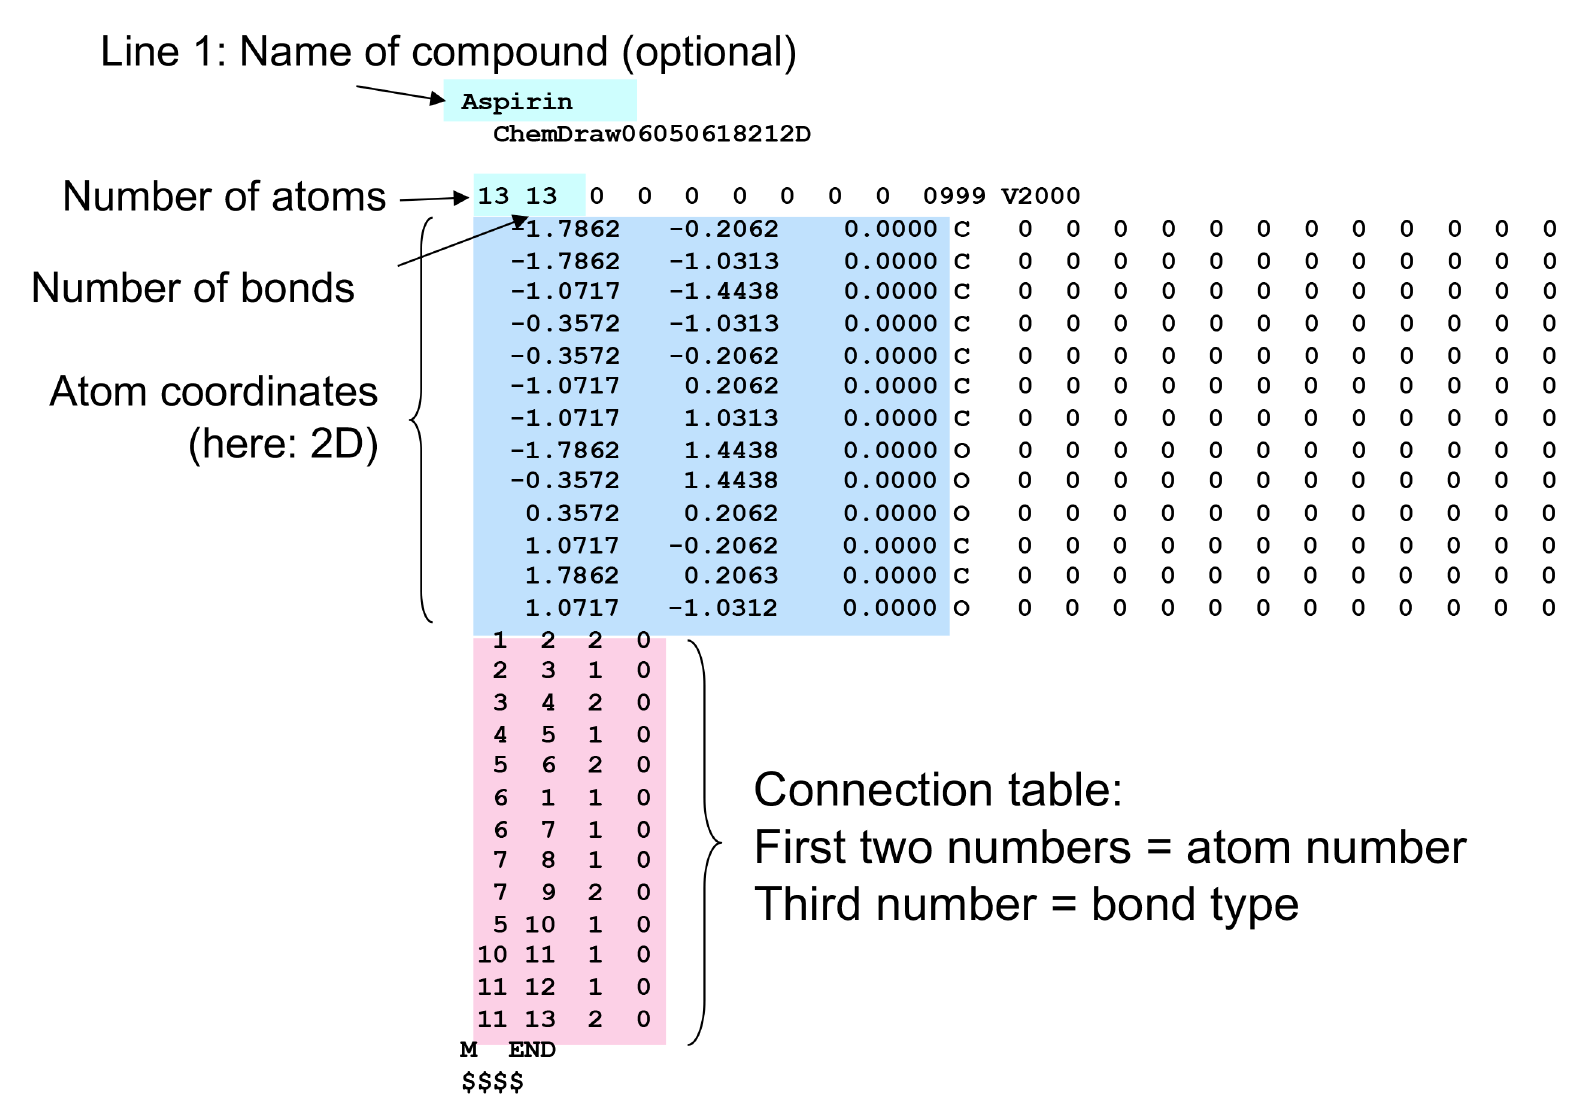
\includegraphics[width=0.70\textwidth]{img/cheminformatics/DataFormat.png}\end{center}

\subsection{1D representation}

The most efficient way to represent molecules for storage is a 1D representation. Furthermore, it can be easily interpreted by a computer and searched in a database. However, it is important that the representation is \emph{reversible}, that the transformations 2D $\rightarrow$ 1D and 1D $\rightarrow$ 2D can be carried out without any problems, and that the representation is \emph{unique}. To achieve this, stereochemistry and aromaticity must be retained in the representation. Examples of such representations are the IUPAC name, WLN, SLN, SMILES and InChI, although we will only deal with the latter two in the following.

\subsubsection{SMILES}

SMILES stands for \emph{Simplified Molecular Input Line Entry System}. It was introduced in 1988 and is based on representing the chemical structure using letters according to established rules. On the computer, a \emph{minimum spanning tree} is first created from a graph, which is then translated into the SMILES using a \emph{depth-first} algorithm, whereby different applicable SMILES are generated depending on which atom is started with. Therefore, a \emph{canonicalization} is needed to make the representation unique. SMILES follows the following rules:

\begin{itemize}
    \item Hydrogens as well as single and aromatic bonds are usually omitted, but can be specified explicitly if desired.
    \item \textbf{Atoms:}
    \begin{itemize}
        \item General: Atomic symbol in square brackets
        \item “Organic” subset (= B, C, N, O, P, S, F, Cl, Br, I) can be written without brackets if the number of attached Hs is “normal”.
        \item Attached hydrogens and formal charges always specified inside brackets.
        \item Atoms in aromatic rings are specified by lower case letters (i.e. c, n).
        \item Stereocentres are specified with @ (anti-clockwise writing of neighbors) and @@ (clockwise writing of neighbors) inside brackets.
    \end{itemize}
    \begin{center}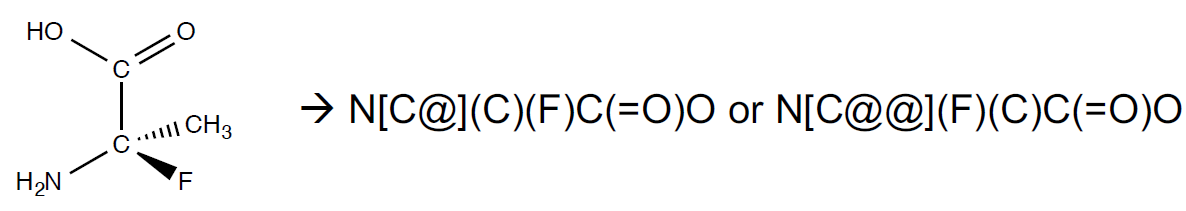
\includegraphics[width=0.65\textwidth]{img/cheminformatics/SmilesRulesAtoms.png}\end{center}
    \item \textbf{Bonds:}
    \begin{itemize}
        \item Single bond: “-”, double bond: “=“, triple bond: "\#" aromatic bond: “:”
        \item Cis/trans double bonds: use of “/” and “$\backslash$”, e.g.
    \end{itemize}
    \begin{center}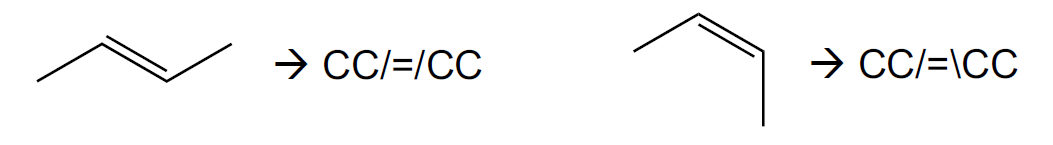
\includegraphics[width=0.65\textwidth]{img/cheminformatics/SmilesRulesBonds.png}\end{center}
    \item \textbf{Branches:}
    \begin{itemize}
        \item Specified by parentheses
        \item Can be nested or stacked
    \end{itemize}
    \begin{center}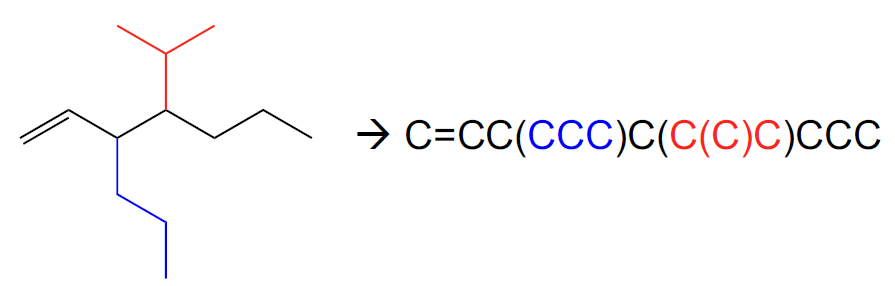
\includegraphics[width=0.65\textwidth]{img/cheminformatics/SmilesRulesBranches.png}\end{center}
    \item \textbf{Cyclic structures:}
    \begin{itemize}
        \item Represented by breaking one bond (to get spanning tree) and numbering the ring-closure atoms
        \item Ring-closure digits can be reused
    \end{itemize}
    \begin{center}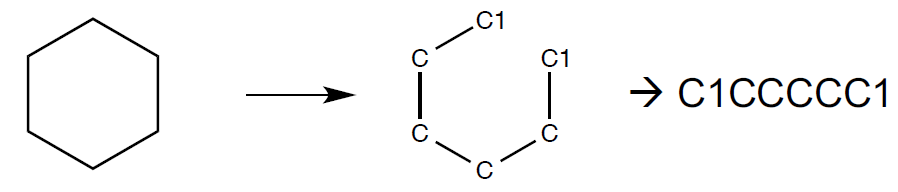
\includegraphics[width=0.65\textwidth]{img/cheminformatics/SmilesRulesCyclic.png}\end{center}
    \item \textbf{Aromaticity}
    \begin{itemize}
        \item Aromaticity in cheminformatics is a concept! Different definitions/algorithms exist (discussed later). Do not confuse it with a physical phenomenon
        \item Aromatic bonds are usually omitted
        \item Atoms in an aromatic ring are specified by lower case letters
    \end{itemize}
    \begin{center}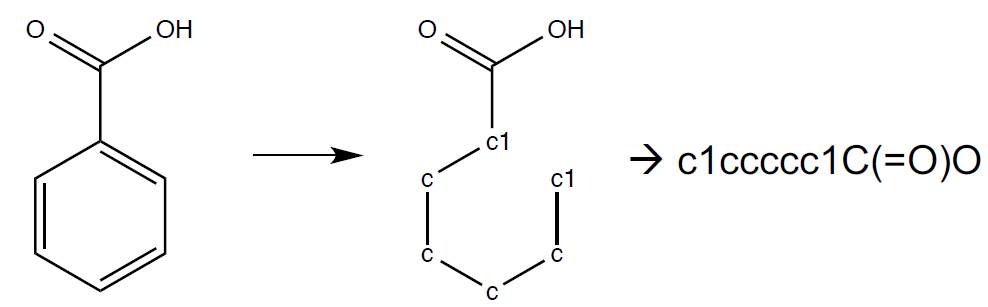
\includegraphics[width=0.65\textwidth]{img/cheminformatics/SmilesRulesAromaticity.png}\end{center}
\end{itemize}

\textcolor{red}{Beispiele aus den slides machen und einfügen.}

% not finished code
%\lstinputlisting[language=C++]{src/cheminformatics/smiles.cpp}

\subsubsection{Canonicalization}

As already mentioned, several correct SMILES can be used for one molecule, depending on which atom you start with. Therefore, a canonicalization must be performed to create a unique and reproducible numbering of the atoms of a molecule.

\deff{Graph Isomorphism}{Two graphs are isomorphic when there is a 1-to-1 mapping (a permutation) from the vertices of one graph to the vertices of the other, such that the edge connections are respected. In short, isomorphic graphs are structurally the same, but the labeling of the vertices is different.}

\deff{Graph Invariant}{In graph theory, a graph property or graph invariant is a property of graphs that depends only on the abstract structure, not on graph representations such as particular labellings or drawings of the graph. Therefore, two isomorphic graphs have the same invariants.}

In the example of cheminformatics, the invariants of a graph are usually a combination of information such as element, number of bonds, number of hydrogens, ring information, etc.

\paragraph{Morgan's Algorithm}
Morgan's algorithm is a canonicalization algorithm for chemical compounds presented in 1965 that uses the number of bonding partners (excluding hydrogen) as invariants. The algorithm proceeds as follows:

\begin{enumerate}
    \item \emph{Step 1: Find invariants}
    \begin{itemize}
        \item First assign the initial invariants to each atom, i.e. the number of bonds.
        \item Then assign new invariants for each atom, which are the sum of the invariants of the neighbors (excluding its own invariant). Repeat this step until the number of invariants no longer increases.
    \end{itemize}
    \begin{center}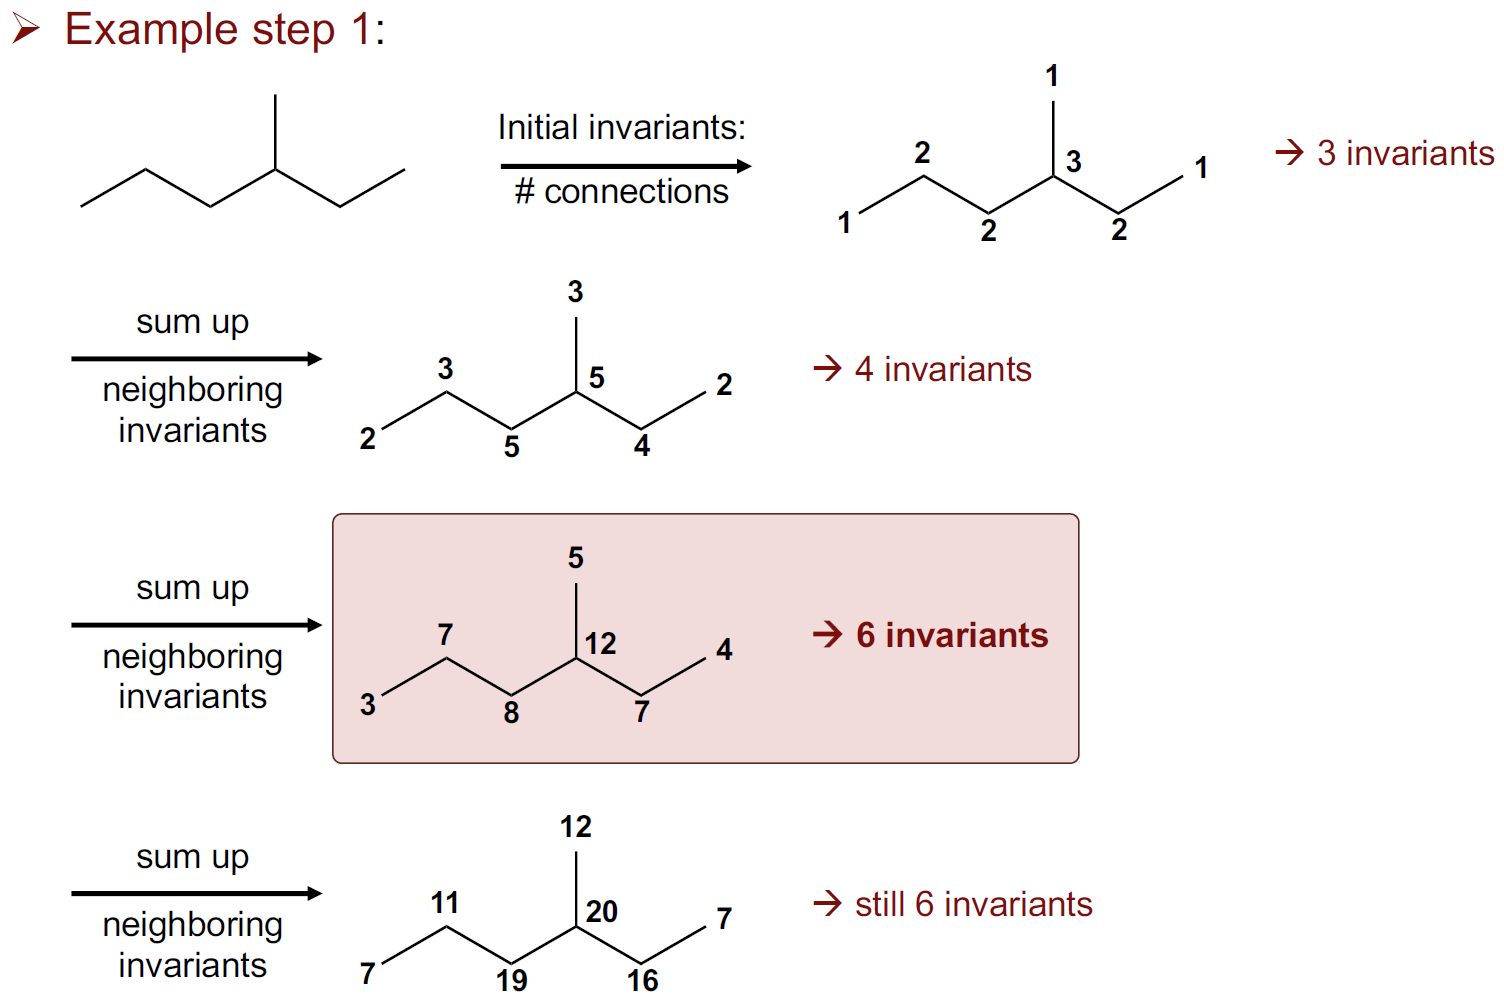
\includegraphics[width=0.85\textwidth]{img/cheminformatics/Morgan1.png}\end{center}
    \item \emph{Step 2: Set ranks}
    \begin{itemize}
        \item Take the graph where the number of invariants increased last time (not the graph where they were increased but the number of invariants remained the same).
        \item Take the largest invariant and set the rank of the atom to 1.
        \item Take the neighbors of the atom with rank 1, order them by descending invariants and give them the ranks 2-4 accordingly (assuming three are bonded).
        \item Now always choose the atom with the smallest rank and assign ranks to its neighbors according to descending invariants. Repeat this step until each atom has a rank.
    \end{itemize}
    \begin{center}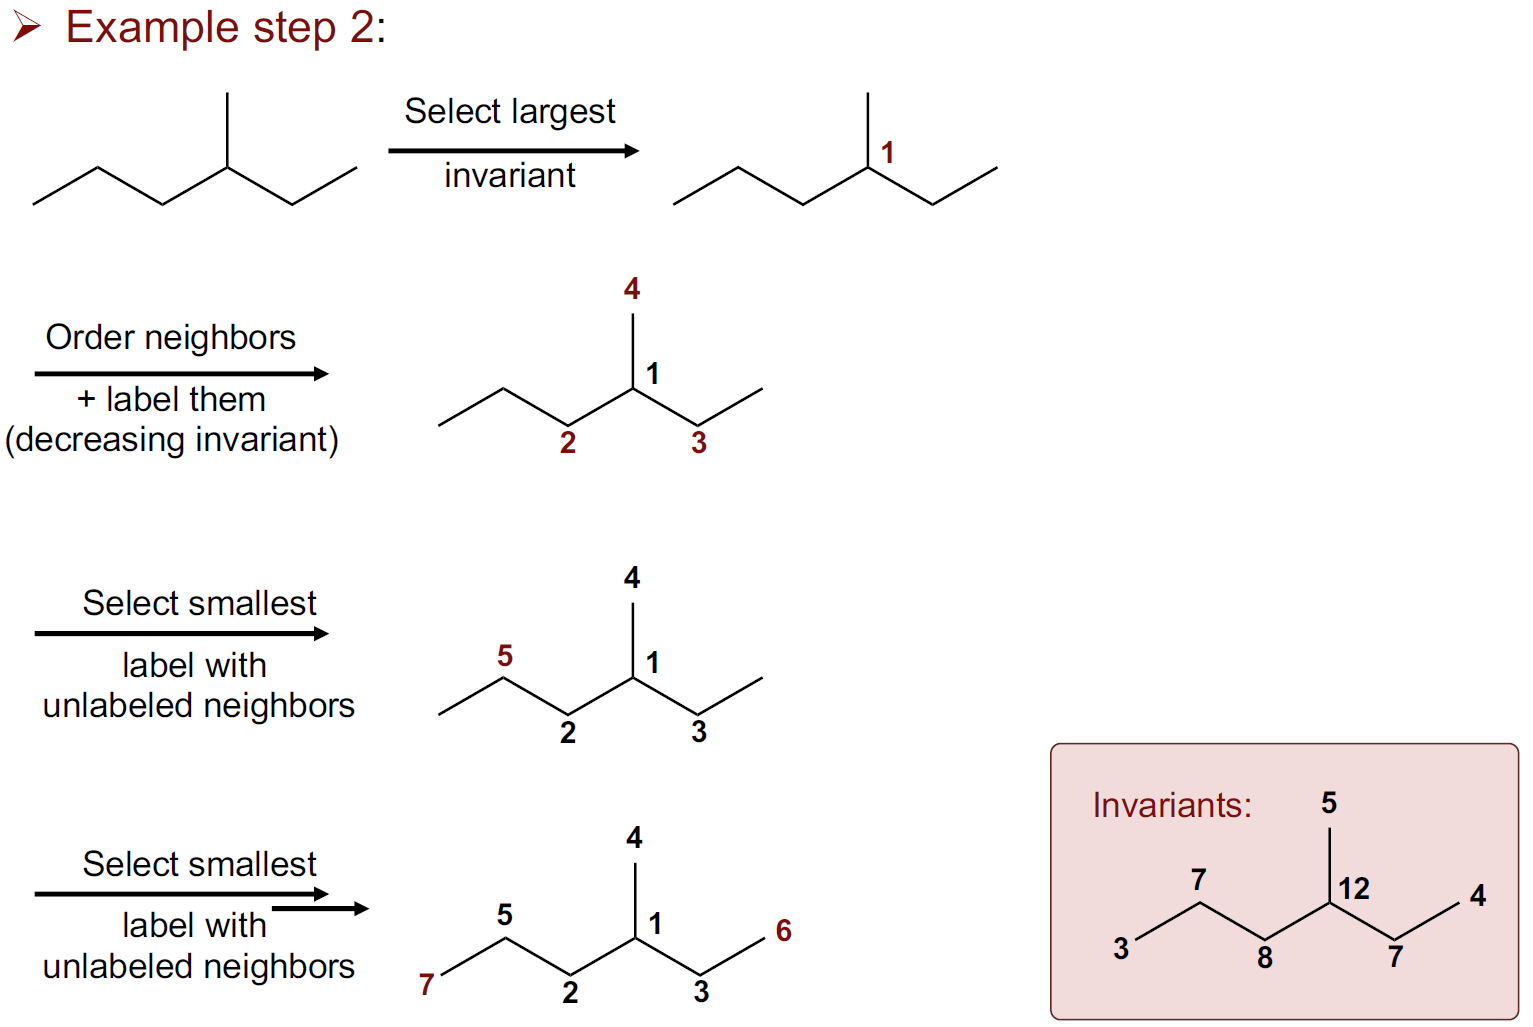
\includegraphics[width=0.85\textwidth]{img/cheminformatics/Morgan2.png}\end{center}
\end{enumerate}

The main criticism of Morgan's algorithm is that the summation step produces ambiguous results, which is why uniqueness cannot be proven. One way to solve this is to also include the atom type and bond multiplicity. Furthermore, oscillations can occur for certain symmetrical molecules, so that the first step has no termination condition.

% not finished code
%\lstinputlisting[language=C++]{src/cheminformatics/morgan.cpp}

\paragraph{Cangen Algorithm}

Just like Morgan's algorithm, CANGEN uses the number of binding partners to find the invariants. However, in the iterative calculation, CANGEN uses the product of primes instead of the sum of the invariants of the neighbors, as in Morgan's algorithm, to minimize ambiguities. However, a unique numbering cannot be proven here either.

\begin{enumerate}
    \item 
\end{enumerate}

% not finished code
%\lstinputlisting[language=C++]{src/cheminformatics/cangen.cpp}

\subsubsection{InChI}

\subsubsection{Ring perception}

The idea behind ring perception is to develop an algorithm that can automatically detect ring structures in 1D representations of molecules. The whole thing must therefore be independent of the projection, orientation and labeling of the ring system.

\begin{itemize}
    \item \textbf{Chords:}
    \begin{itemize}
        \item Minimum number of bonds whose removal is required to turn a structure from cyclic to acyclic.
    \end{itemize}
    \item \textbf{Nullity:}
    \begin{itemize}
        \item Number of chords that can be calculated using the formula below, where components stands for the number of closed graphs (always 1 for a molecule).
    \end{itemize}
    \begin{align}
        \mu=\#_\mathrm{bonds}-\#_\mathrm{atoms}+\#_\mathrm{components}
    \end{align}
    \item \textbf{Cycle:}
    \begin{itemize}
        \item Traversable node by node in a single path back to the start.
    \end{itemize}
\end{itemize}

The size we now want to determine exactly is the smallest set of smallest rings (SSSR), in which as many rings of the smallest possible size as possible are found. 

\begin{center}
    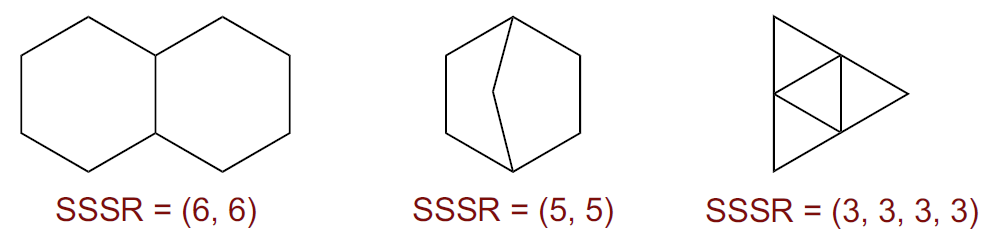
\includegraphics[width=0.85\textwidth]{img/cheminformatics/RingPerceptionSssr.png}
\end{center}

\paragraph{Figueras' algorithm}
Figueras' algorithm is an algorithm presented in 1996 to determine the SSSR of a molecule. The algorithm proceeds as follows:

\begin{enumerate}
    \item 
\end{enumerate}

\begin{center}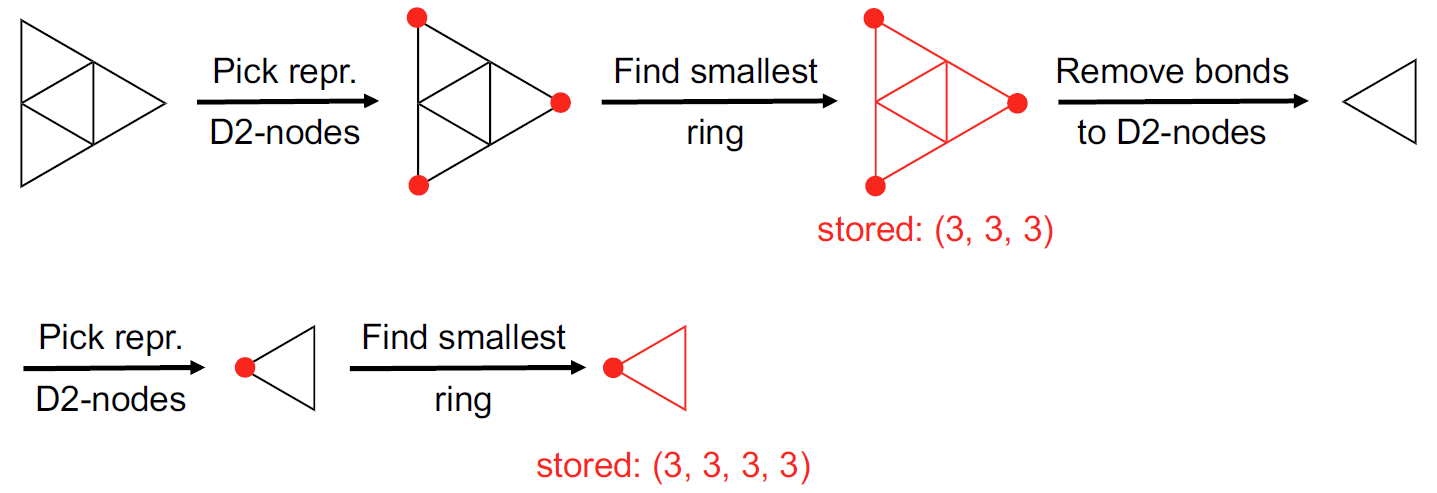
\includegraphics[width=0.85\textwidth]{img/cheminformatics/RingPerceptionFigueras1.png}\\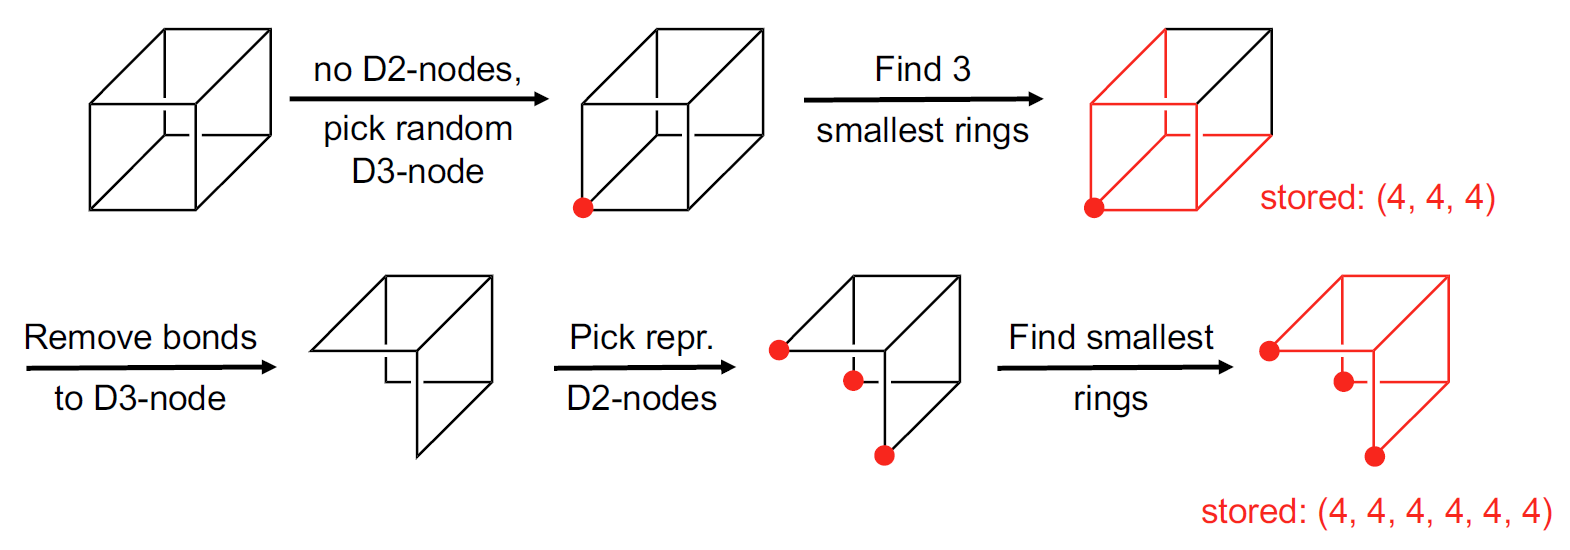
\includegraphics[width=0.85\textwidth]{img/cheminformatics/RingPerceptionFigueras2.png}\end{center}

% not finished code
%\lstinputlisting[language=C++]{src/cheminformatics/figueras.cpp}

\subsubsection{Aromaticity detection}

The definition of armoaticity is not trivial and the implementation in cheminformatics is still under discussion, because for cheminformatics a definition has to be found that is as simple as possible, that applies in most cases and is co-agent with SMILES and substructure search. Therefore, the cheminformatics definition does not necessarily imply physical properties of the molecule.

\begin{itemize}
    \item \textbf{Hückel's rule:}
    \begin{itemize}
        \item $(4n+2)\;\pi$-electrons $\rightarrow$ aromatic
    \end{itemize}
    \item \textbf{Extension of Hückel’s rule:}
    \begin{itemize}
        \item $(4n+2)\;\pi$-electrons and all atoms $\mathrm{sp}^2$ (planar) $\rightarrow$ aromatic
    \end{itemize}
\end{itemize}

With SMILES, both the Kekulè form (localized double bonds) can be used, as well as the explicit labeling of aromaticity with lowercase letters, whereby the latter is the preferred output of SMILES, since the former creates an artificial asymmetry.

\begin{align*}
    &\textit{Exapmle: benzene}&\begin{cases}
        \textit{Kekulè: }&\text{C1=CC=CC=C1}\\
        \textit{SMILES: }&\text{c1ccccc1}
    \end{cases}
\end{align*}

Aromatic systems over several rings are generally more difficult. For example, non-aromatic single bonds between two aromatic rings should be explicitly written with “-” in SMILES (e.g. biphenyl with c1ccccc1-c2ccccc2).

\paragraph{Aromaticity in the RDKit:}
The RDKit uses the Hückel rule for aromaticity, whereby a ring or condensed ring system with $(4n+2)\;\pi$-electrons is considered aromatic. Both bonds and atoms can be aromatic, whereby an aromatic bond must be between two aromatic atoms, but a bond between two aromatic atoms does not necessarily have to be aromatic. This is why in condensed ring systems the individual cycle can be not aromatic, but the overall system is.

\begin{center}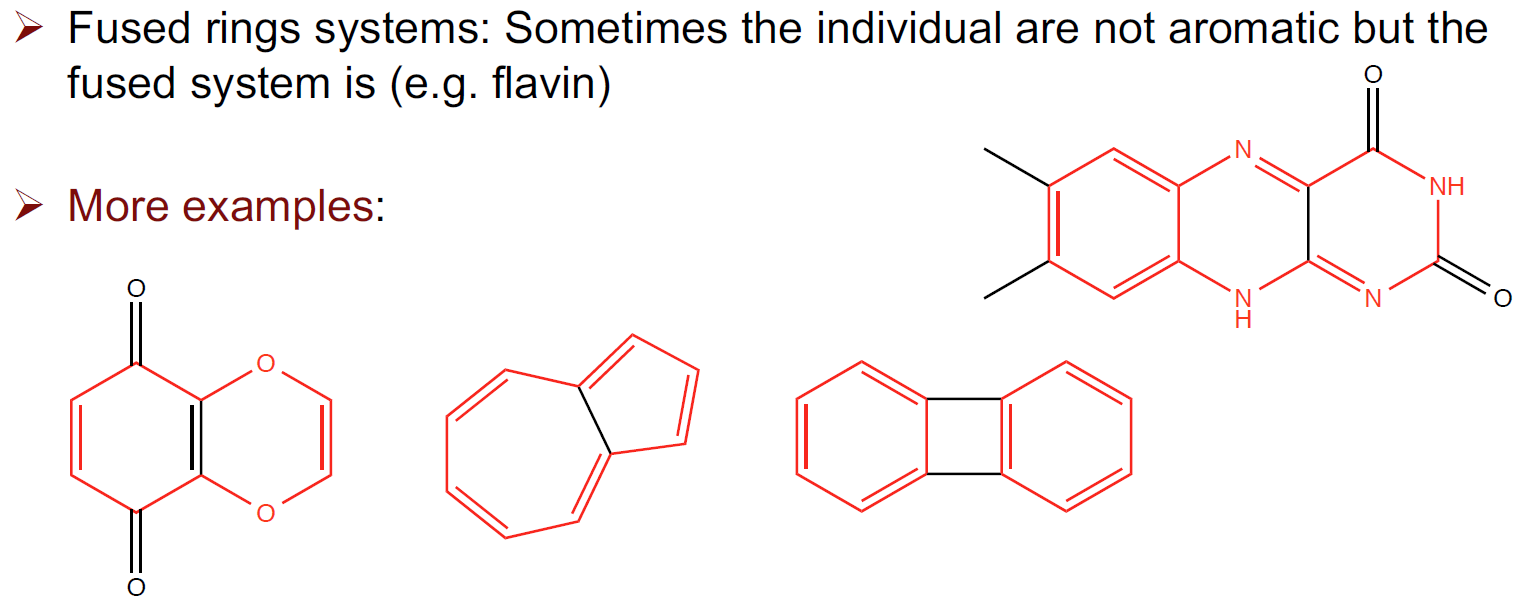
\includegraphics[width=0.85\textwidth]{img/cheminformatics/AromaticRdkit.png}\end{center}

\subsection{Substructure search}

In cheminformatics, a distinction is made between three shifting structure searches:

\begin{itemize}
    \item \textbf{Full structure search:}
    \begin{itemize}
        \item Question: Is this molecule in my database?
        \item Input: Full chemical structure (e.g. SMILES)
        \item Solution: Comparison of SMILES, InChi (keys), internal index number, etc.
    \end{itemize}
    \item \textbf{Substructure search:}
    \begin{itemize}
        \item Question: Does this substructure exist in any molecule of my database?
        \item Input: Query pattern of atoms and bonds (e.g. SMARTS).
        \item Solution: Brute-force, backtracking, partitioning and relaxation
    \end{itemize}
    \item \textbf{Superstructure search:}
    \begin{itemize}
        \item Question: Are any molecules in my database substructures of the query?
        \item Input: full chemical structure (e.g. SMILES)
        \item Solution: same as substructure search
    \end{itemize}
\end{itemize}

\subsubsection{SMARTS}

SMARTS (SMILES arbitrary target specification) is an extension of the classic SMILES to describe molecular patterns (substructures). With SMILES only exact atoms can be specified, whereas with SMARTS wildcards for atoms and bonds are possible, which can simplify the substructure search.

\begin{itemize}
    \item \emph{Atoms:}
    \begin{itemize}
        \item Specified by either element symbol or number: e.g. [\#6] $\rightarrow$ any carbon
        \item “*” : wild card
        \item “A” : any aliphatic atom
        \item “a” : any aromatic atom
        \item “D” followed by a number : degree (number of explicit connections)
        \item “R” followed by a number n : in n smallest rings
        \item “r” followed by a number n : in a smallest ring of size n
        \item “H” followed by a number : number of adjacent hydrogens
        \item H has now two meanings: e.g. [H] $\rightarrow$ hydrogen atom, [*H2] $\rightarrow$ any atom with two hydrogens
        \item Multiple possible matches are separated by a comma: e.g. [C,N] $\rightarrow$ either aliphatic C or N
    \end{itemize}
    \item \emph{Bonds:}
    \begin{itemize}
        \item “$\sim$” : any bond
        \item “@” : any ring bond
    \end{itemize}
    \item \emph{Logical operators:} combinations of atom and bond specifications
    \begin{itemize}
        \item “!” : NOT, e.g. [!C] $\rightarrow$ not aliphatic carbon
        \item “\&” : AND (high priority)
        \item “,” : OR
        \item “;” : AND (low priority)
        \item Operator priority: “!” > “\&” > “,” > “;”
    \end{itemize}
    \item \emph{Aromaticity:}
    \begin{itemize}
        \item Note: a double bond is not matched to an aromatic bond!
    \end{itemize}
\end{itemize}

\begin{center}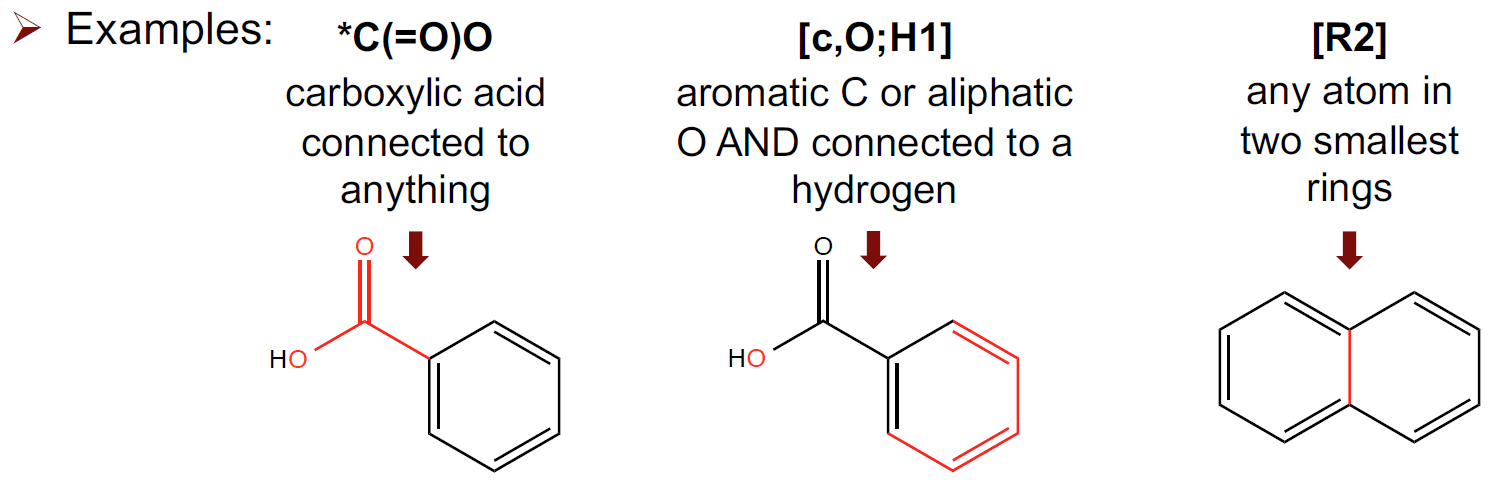
\includegraphics[width=0.85\textwidth]{img/cheminformatics/SubstructureSmartsExample.png}\end{center}

Algorithmically, however, such a search is not easy to program. If we consider the problem of checking whether two graphs are isomorphic, this algorithm already scales with $\Theta(N!)$, where $N$ is the number of nodes in the graph. In this brute-force algorithm (depth-first tree search), a 1-to-1 mapping is made so that each node from $G_1$ is mapped against an unmapped node from $G_2$ and it is checked whether all neighbors are equal. It is assumed that graph isomorphism is an \emph{NP-complete} problem, but this has not yet been proven rigerously.

\deff{Subgraph isomorphism}{The subgraph isomorphism problem is a generalization of graph isomorphism, where the question is whether $G_1$ is a subgraph of $G_2$. In the worst case this is an NP-complete problem, but average running time is much better than for the classical graph isomorphism problem. In addition, heuristics can be used for molecular graphs, which also reduce the running time (bounded valence and bond multiplicity)}

In general, there are the following algorithms for substructure search:

\begin{itemize}
    \item \emph{Backtracking}
    \begin{itemize}
        \item Rax and Kirsch \shortrefurl{Science}{1975}{126}{814-819}{https://doi.org/10.1126/science.126.3278.814}
    \end{itemize}
    \item \emph{Partitioning and relaxation (often combined with backtracking)}
    \begin{itemize}
        \item Sussenguth’s partitioning algorithm \shortrefurl{J. Chem. Docum.}{1965}{5}{36-43}{}
        \item Figueras’ set reduction algorithm \shortrefurl{J. Chem. Docum.}{1972}{12}{237-244}{}
        \item Ullmann’s algorithm \shortrefurl{J. Assoc. Comput. Mach.}{1976}{23}{31-42}{}
        \item von Scholley’s relaxation algorithm \shortrefurl{J. Chem. Inf. Comput. Sci.}{1984}{24}{235-241}{}
        \item vf2 and variants \shortrefurl{IEEE Trans Pattern Analysis Machine Intelligence}{2004}{26}{1367-1372}{}
    \end{itemize}
\end{itemize}

In the worst case, the running time is still exponential, but that doesn't happen often.

\subsubsection{Backtracking (Ray and Kirsch)}

Backtracking uses a depth first algorithm (for the searching tree) to map one graph of the pattern (substructure) against the graph of the full molecule. As soon as a branch is no longer possible, it is backtracked to an atom where a solution is still possible.

\begin{enumerate}
    \item Map arbitrary pair of nodes.
    \item Map neighbors of these nodes.
    \item If successful repeat step 2, if not backtrack to step 1 and choose another pair (query atom stays the same).
\end{enumerate}

The algorithm is terminated when either all atoms of the pattern have been successfully mapped (MATCH) or all mapping attempts of the first query node fail (NO MATCH). You can speed up the algorithm somewhat by, for example, only mapping nodes with the same element, charge and number of bonds against each other, or by starting with unusual atoms with many bonds, because then the probability of recognizing a mismatch earlier is higher.

\begin{center}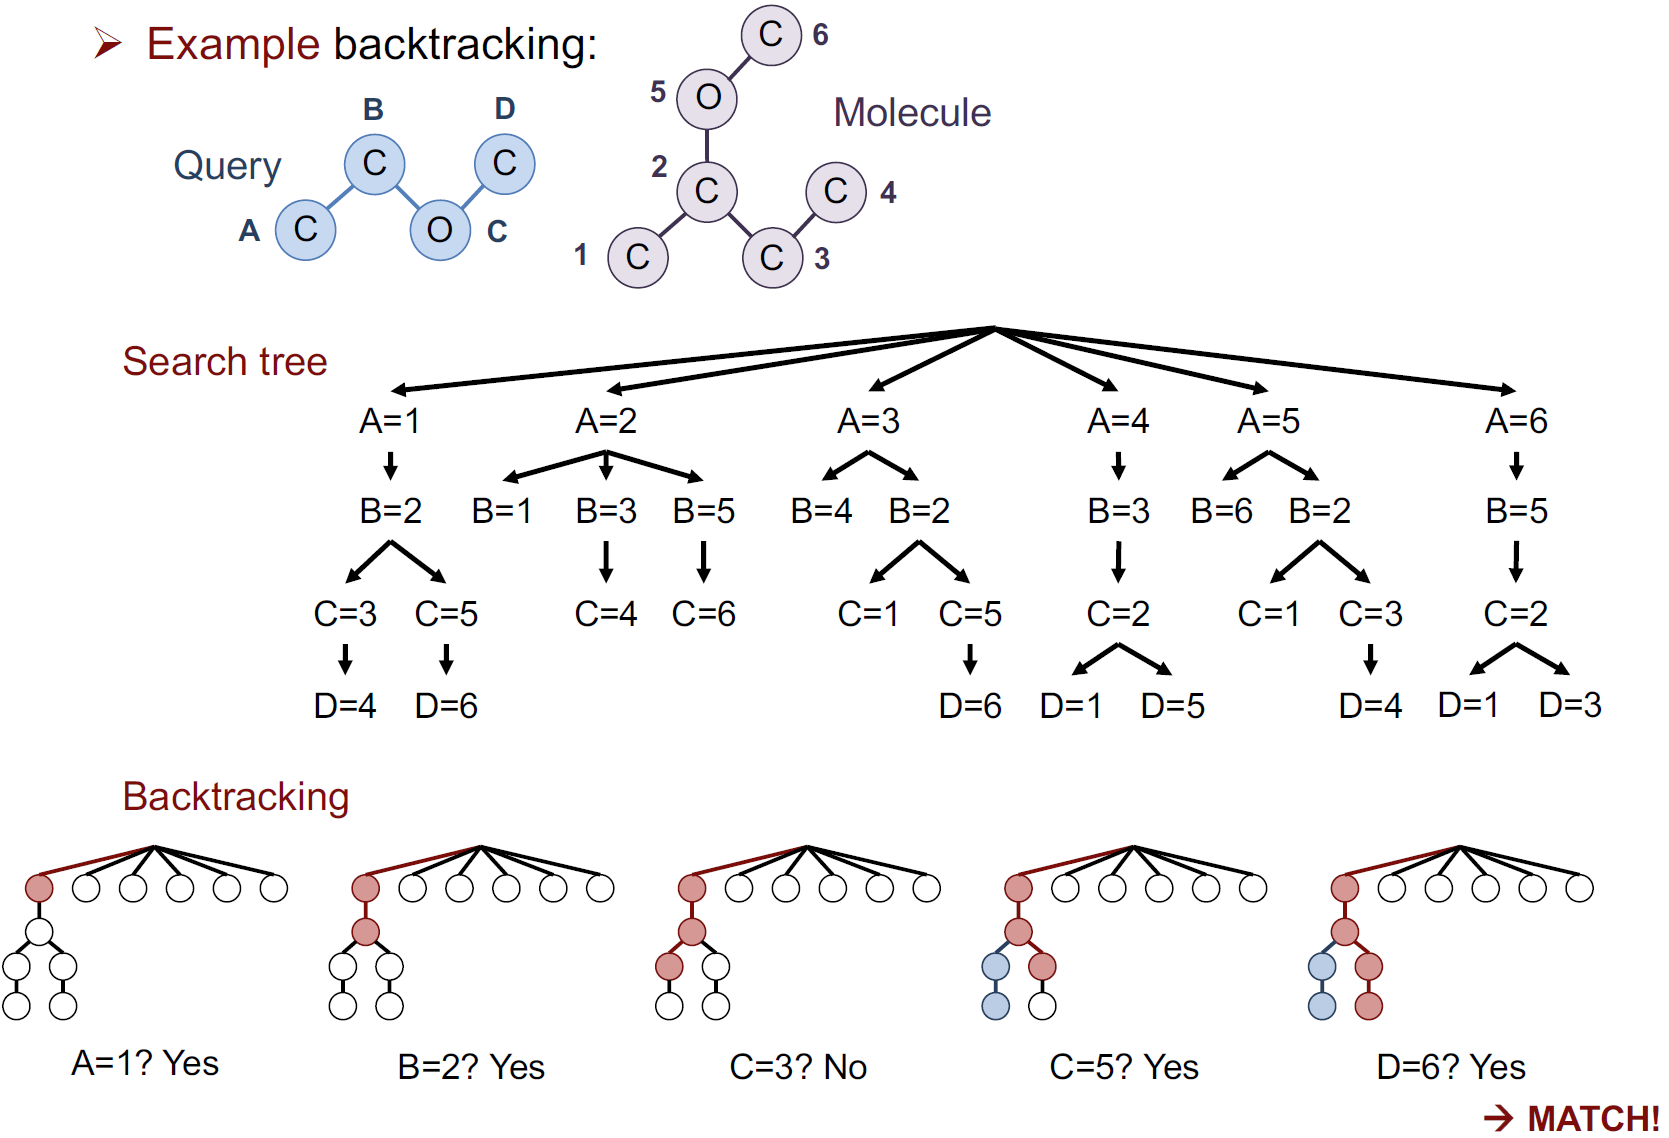
\includegraphics[width=0.85\textwidth]{img/cheminformatics/SubstructureBacktracking.png}\end{center}

\subsubsection{Partitioning and relaxation (Ullmann's algorithm)}

\begin{itemize}
    \item \textbf{Partitioning}
    \begin{itemize}
        \item Divide nodes of each graph into subsets of potential correspondents based on atom labels (e.g. N can only match N of number of connections).
    \end{itemize}
    \item \textbf{Relaxation}
    \begin{itemize}
        \item Label of a node is enhanced by examining its immediate neighbors.
    \end{itemize}
\end{itemize}

Ullmann's algorithm is a combination of a depth-first backtracking procedure and a relaxation step in between. During the algorithm, an $N_\mathrm{query}$ row by $N_\mathrm{structure}$ column bool-matrix is optimized, which stores whether atoms of the pattern map to atoms of the molecule. You can speed up the algorithm a little by starting with rare elements or atoms with many connections. The algorithm proceeds as follows:

\begin{enumerate}
    \item We first set up the original matrix $M_0$ by looking at each row (each atom of the pattern) to see if each atom of the molecule has at least as many connections as the atom of the pattern (Yes = 1, No = 0). Therefore, the atoms $A$, $C$ and $E$, which only have one connection, initially match every atom in the structure, since every atom in the structure has at least one connection. Conversely, $B$ with 3 connections only matches atom 4.
    \begin{center}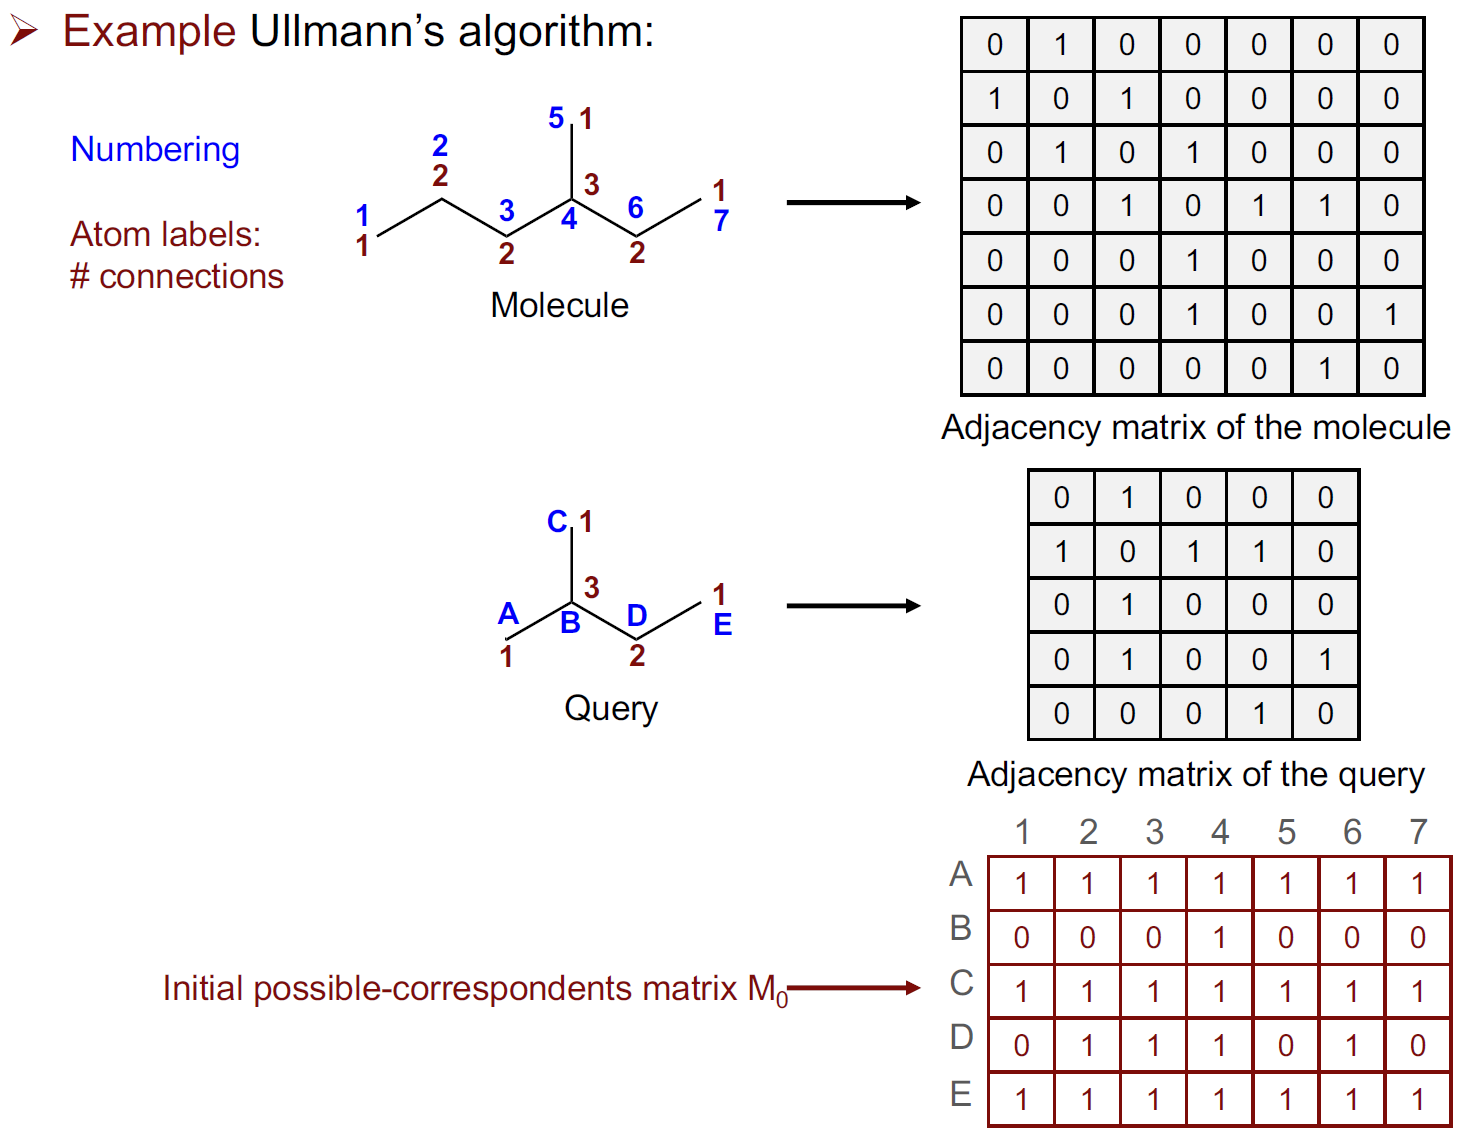
\includegraphics[width=0.85\textwidth]{img/cheminformatics/UllmannInitialMatrix.png}\end{center}
    \item Now the relaxation step follows for each query atom. For this, all neighbors of the corresponding query atom are listed (for $A$ only $B$). Then, for the neighbors, the atoms in the structure that map for the neighbors are looked up in the matrix $M$ (for $B$ only 4). Then, all neighbors for the atoms found in the structure are listed (for 4, these are atoms 3, 5, and 6). Finally, all entries in the matrix for $A$ except 3,5,6 are set to zero.
    \begin{center}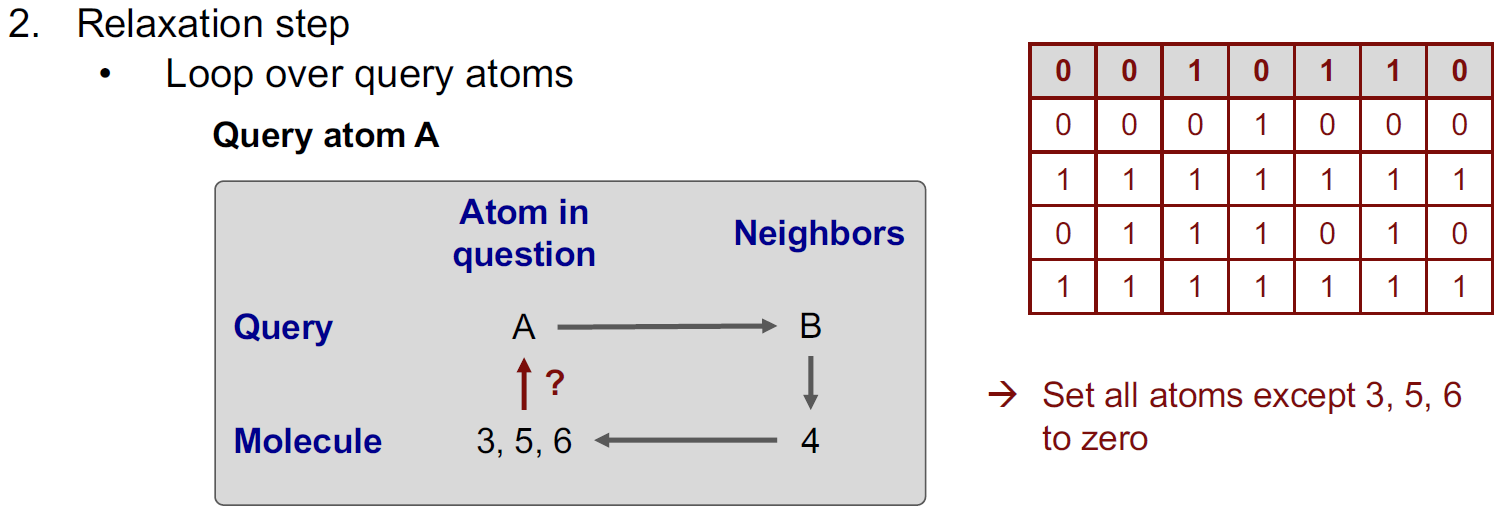
\includegraphics[width=0.85\textwidth]{img/cheminformatics/UllmannRelaxationA.png}\\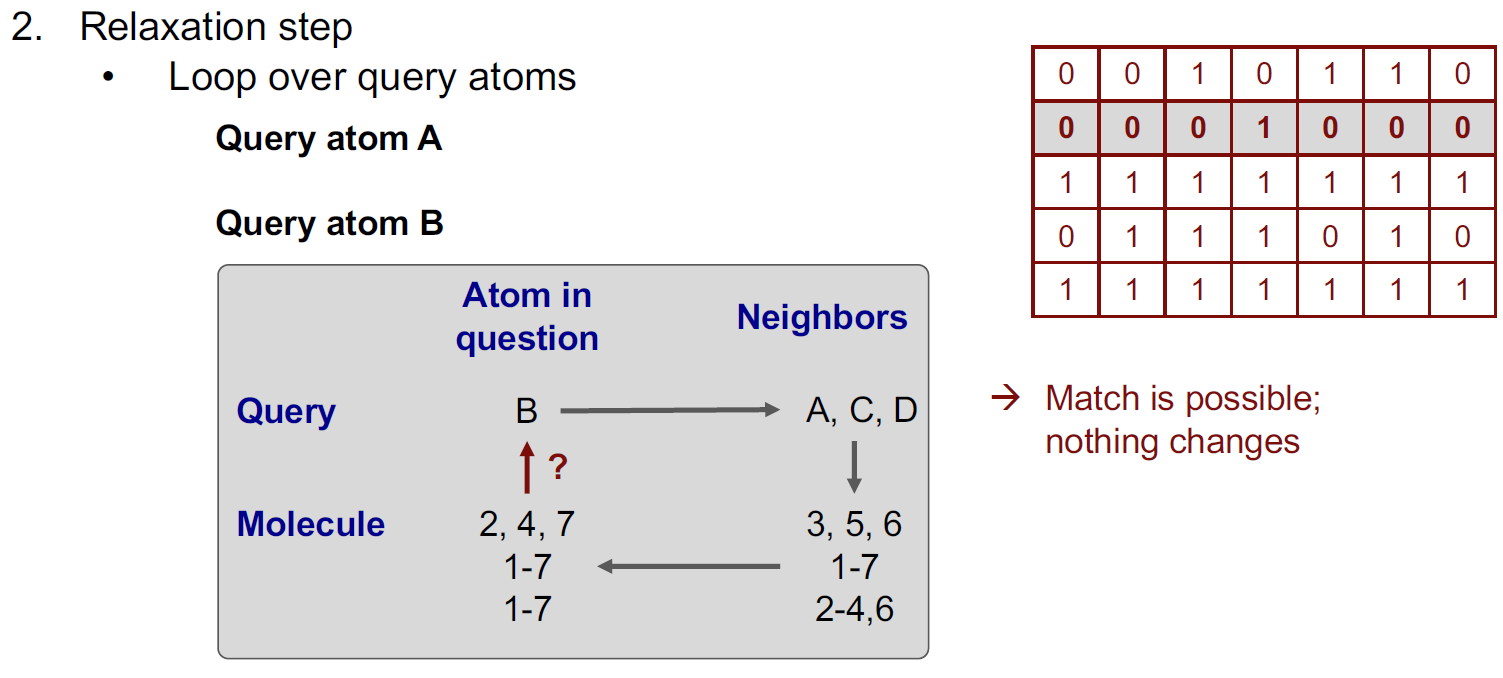
\includegraphics[width=0.85\textwidth]{img/cheminformatics/UllmannRelaxationB.png}\\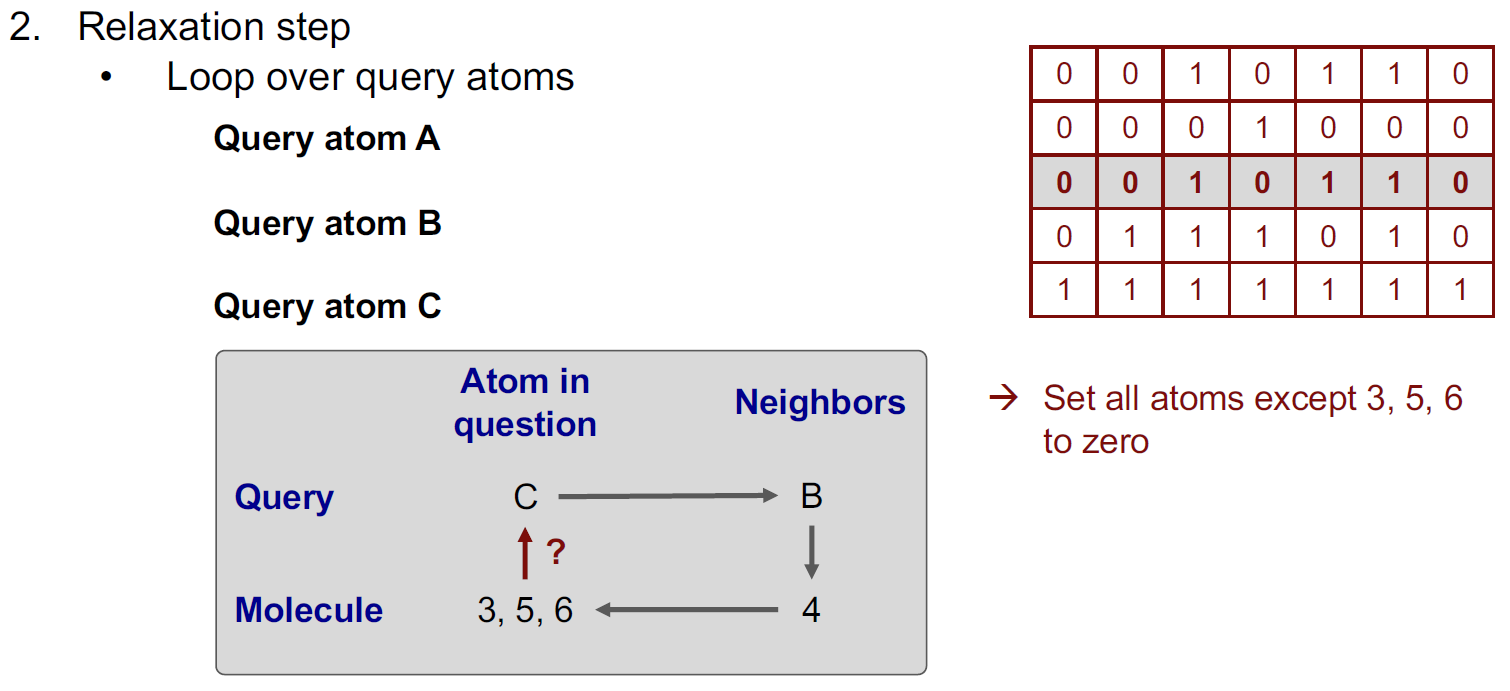
\includegraphics[width=0.85\textwidth]{img/cheminformatics/UllmannRelaxationC.png}\\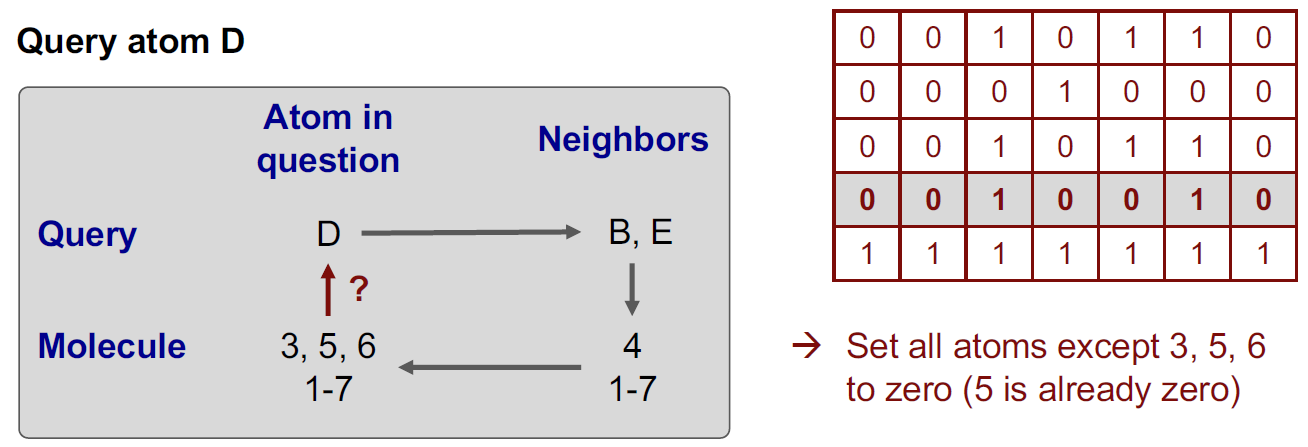
\includegraphics[width=0.85\textwidth]{img/cheminformatics/UllmannRelaxationD.png}\\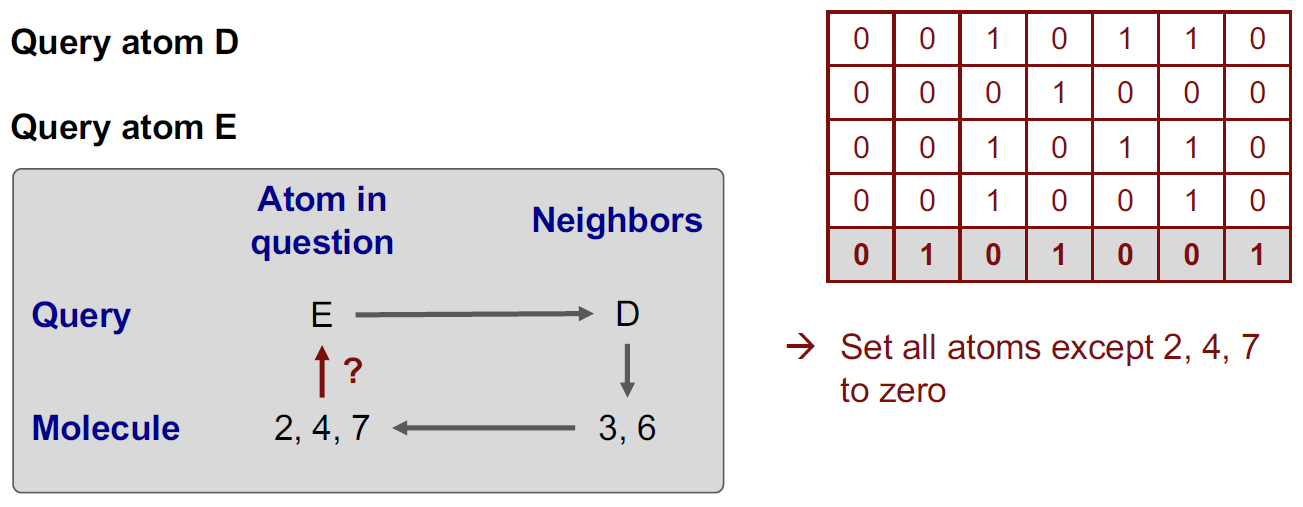
\includegraphics[width=0.85\textwidth]{img/cheminformatics/UllmannRelaxationE.png}\end{center}
    \item We will now start with the backtracking steps. For this, we use a depth-first backtracking algorithm. First, we start with an arbitrary pair of vertices that we assume map. These must of course have a 1 in the matrix $M$ and all other entries in the row and column of the pair are set to 0.
    \begin{center}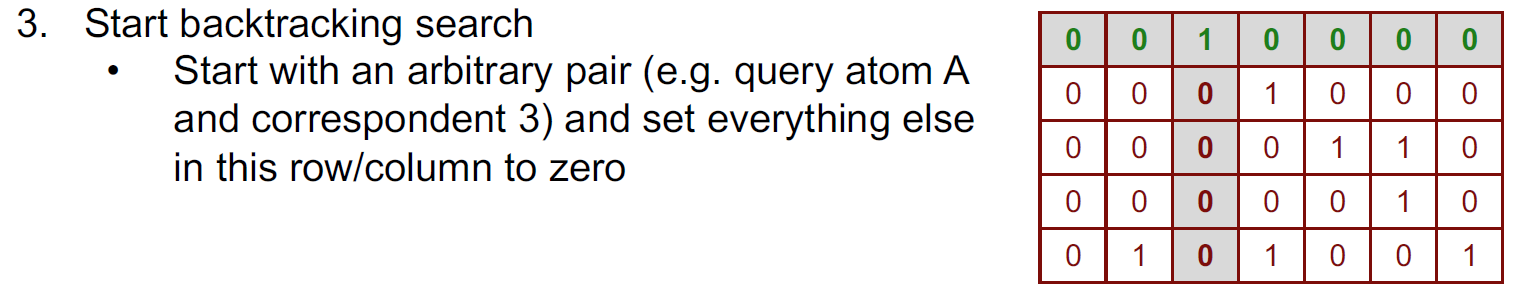
\includegraphics[width=0.85\textwidth]{img/cheminformatics/UllmannBacktrackingA.png}\end{center}
    \item After each backtracking step, the program loops again over each query atom and executes the same algorithm as above to exclude those atoms that have become impossible due to the mapping from A to 3.
    \begin{center}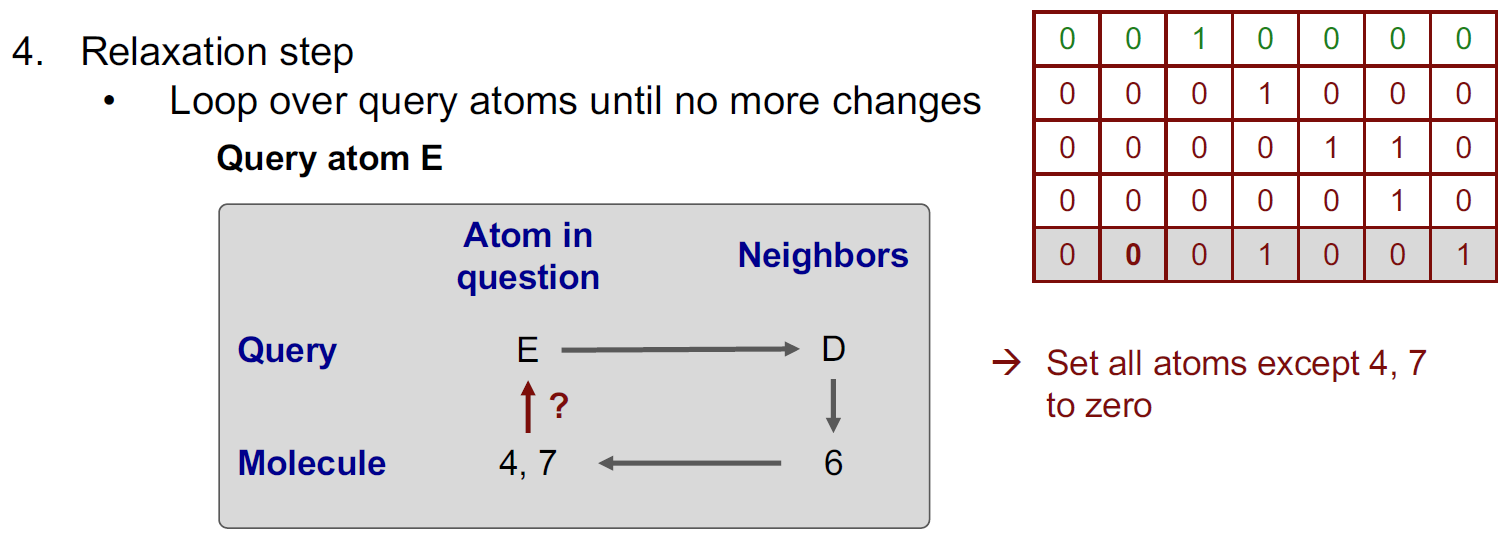
\includegraphics[width=0.85\textwidth]{img/cheminformatics/UllmannBacktrackingAr.png}\end{center}
    \item After that, backtracking and relaxation continue. For $B$, there is only one possible mapping with 4, so it does not change the matrix. For $C$, two atoms are possible, so one is selected and if this selection does not lead to a final match, it is backtracked to.
    \begin{center}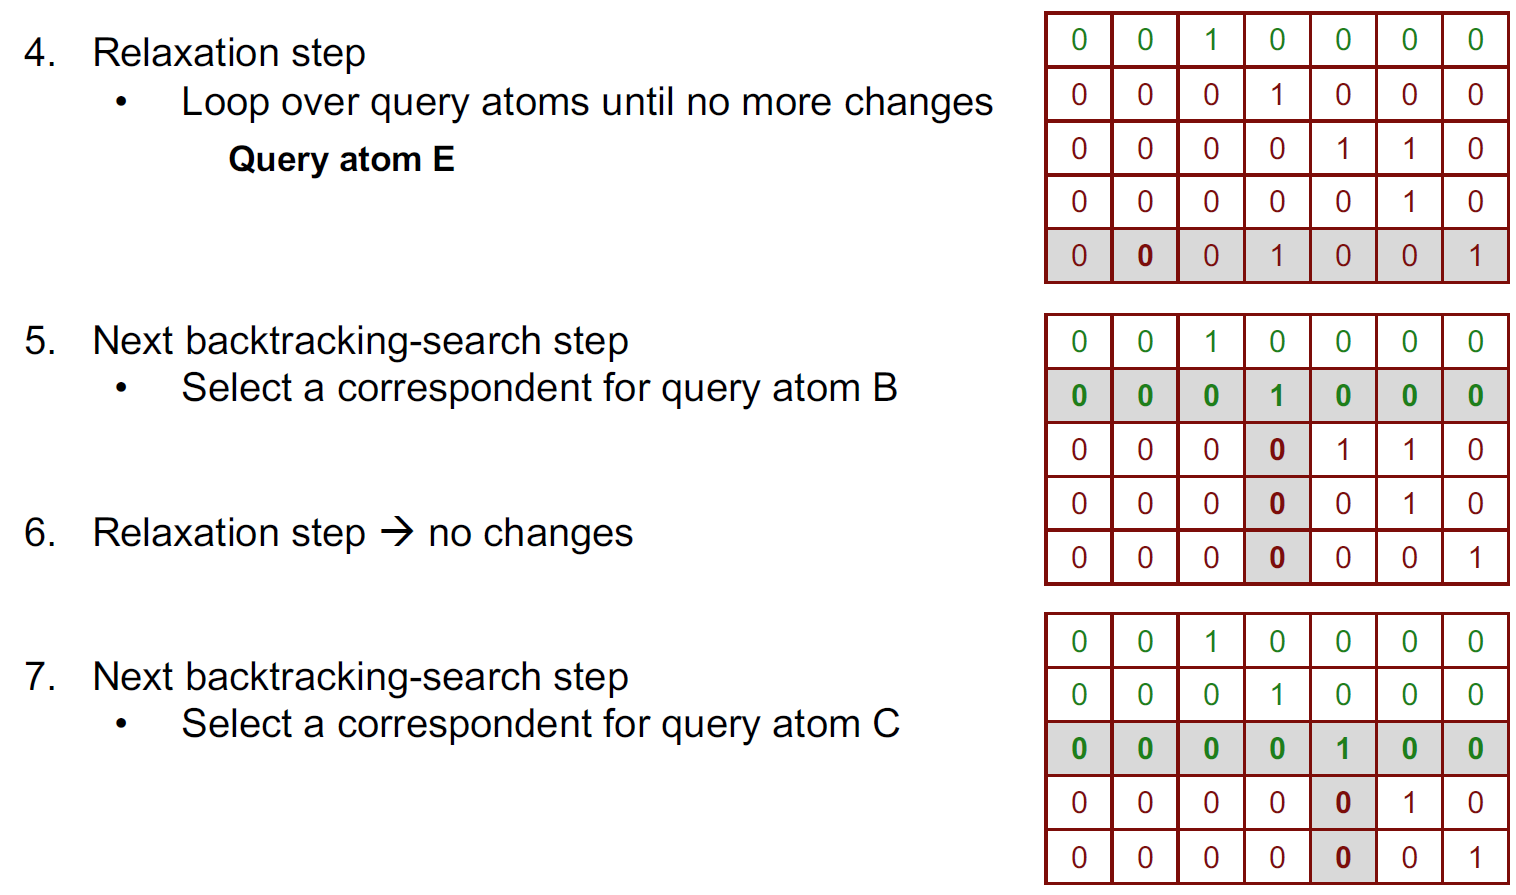
\includegraphics[width=0.85\textwidth]{img/cheminformatics/UllmannBacktrackingB.png}\end{center}
    \item This is done until each line contains only a 1, which indicates a match.
    \begin{center}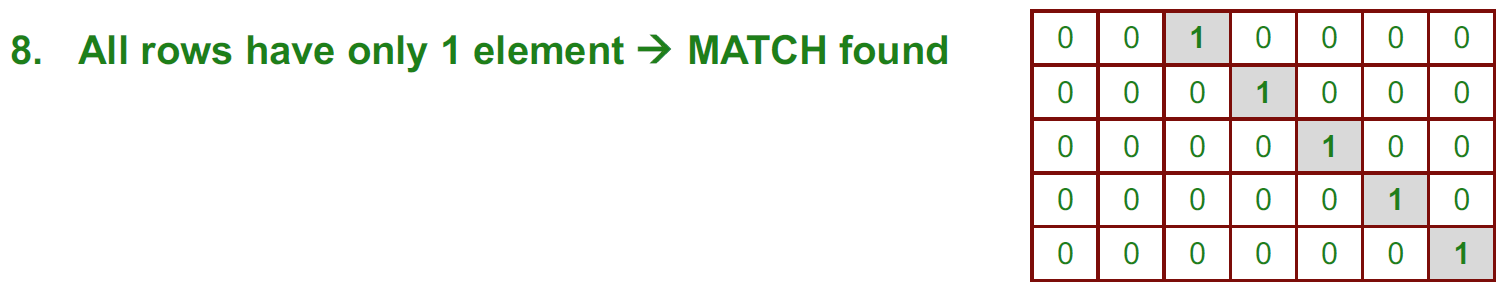
\includegraphics[width=0.85\textwidth]{img/cheminformatics/UllmannBacktrackingC.png}\end{center}
\end{enumerate}

% not finished code
%\lstinputlisting[language=C++]{src/cheminformatics/ullmann.cpp}

\subsubsection{Molecular fingerprints}

However, Ullmann's algorithm is still too slow to search for structures in larger databases, which is why molecular fingerprints are introduced. For this purpose, the substructure search is divided into two parts:

\begin{enumerate}
    \item Large scale search using molecular fingerprints (bit strings).
    \item Substructure search only for molecules with matching fingerprints.
\end{enumerate}

The idea behind fingerprints is to convert structures into 1D bit strings, where each bit represents a specific fragment that the molecule contains (=1) or does not contain (=0). The advantage is that it is a very compact representation, but it is not unique for complex molecules. Before doing a search generate the substructure fingerprint for the query molecule, FP(query) and then compare FP(query) to FP(mol) for each mol in the database. If every bit in FP(query) is also set in FP(mol), then you need to check for a substructure match between query and mol. Otherwise you can skip it. With a good substructure fingerprint this can eliminate $>99\%$ of the work for typical queries. There are four types of fingerprints based on 2D structures:

\begin{itemize}
    \item \textbf{Dictionary-based}
    \begin{itemize}
        \item Predefined set of substructures (keys)
        \item Bit position directly connected to a certain pattern
        \item Example: Molecular ACCess System (MACCS) from MDL $\rightarrow$ 166 structural keys as SMARTS (Bit 13: “[$\#$8]$\sim$[$\#$7]($\sim$[$\#$6])$\sim$[$\#$6]”)
        \item Example: PubChem fingerprint 1 $\rightarrow$ 881 structural keys (Bit 29: 2 Si, Bit 123: 2 saturated or aromatic carbon-only ring size 3)
    \end{itemize}
    \item \emph{Hashing}
    \begin{itemize}
        \item In path-based, circular and pharmacophore fingerprints patterns are normally hashed to bit positions.
        \item Collisions can occur (different patterns hashed to the same bit position)
    \end{itemize}
    \item \textbf{Path-based}
    \begin{itemize}
        \item Search for all occurrences of a set of generic substructure patterns in the molecule
        \item Example: RDKit fingerprint with patterns with subgraphs with $1-7$ bonds (with hashing)
        \item Example: Atom-pairs fingerprint
    \end{itemize}
    \begin{center}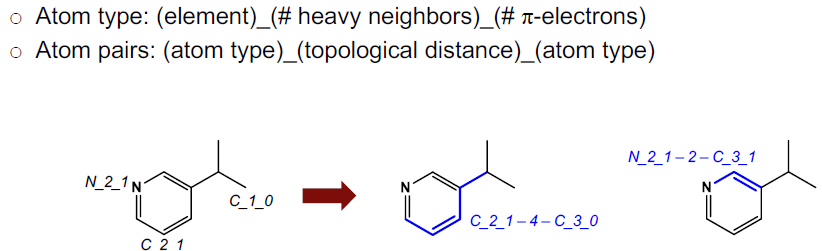
\includegraphics[width=0.85\textwidth]{img/cheminformatics/FingerprintsPathBased.png}\end{center}
    \item \textbf{Circular fingerprints (Morgan fingerprints)}
    \begin{itemize}
        \item Fragments = circular environments around the atoms with different radii
        \item Circular environments hashed to bit positions
        \item Example: Extended connectivity fingerprints (ECFP)
    \end{itemize}
    \begin{center}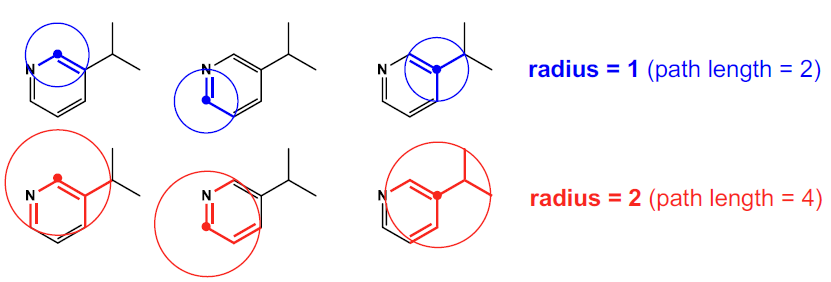
\includegraphics[width=0.85\textwidth]{img/cheminformatics/FingerprintsCircular.png}\end{center}
    \item \textbf{2D pharmacophores}
    \begin{itemize}
        \item Official definition: \emph{Ensemble of steric and electronic features that is necessary to ensure the optimal supramolecular interactions with a specific biological target structure and to trigger (or to block) its biological response}
        \item Pharmacophoric features: H-bond donors/acceptors, hydrophobic, pos./neg. charged, aromatic and/or hydrophobic groups: usually a group of atoms mapped to a virtual point.
        \item 2D pharmacophore fingerprints: Combination of pharmacophoric features and the topological distance between them.
    \end{itemize}
\end{itemize}

\paragraph{Problems}
The main technical problem with fingerprints is that most molecules have only a very small number of fingerprints out of a very large number of possible fingerprints, so most molecules' fingerprints waste a lot of memory space on zero bits. There are two approaches to solving this problem. One is to use \emph{sparse integer vectors} to store only the on-bits. The other is to introduce a second hashing, which, however, can lead to new collisions.

\paragraph{Similarity metrics}
Finally, the actual comparison of the fingerprints must also be implemented efficiently. Either all bits match (value = 1) or no bits match (value = 0). If you want to grade the similarity more finely, you can introduce the \emph{Tanimoto coefficient} $\mathrm{sim}_\mathrm{Tanimoto}$.

\begin{align}
    &\mathrm{sim}_\mathrm{Tanimoto}=\frac{N_{A\&B}}{N_{A}+N_{B}-N_{A\&B}}&\begin{cases}
        N_X&\textit{number of on-bits in fingerprint X}\\
        N_{A\&B}&\textit{number of common on-bits in A and B}
    \end{cases}
\end{align}

The actual comparison operations of the bits are to be introduced using binary LOGIC via AND OR and XOR.

\subsection{Chemical reactions}

Other cheminformatic tasks such as reaction classification, virtual chemical space or reaction prediction cannot avoid the digital representation of chemical reactions in addition to chemical structures, and also mapping atoms on the reactant and product side. Analogous to MOL or SDF files, reactions can be saved in the RXN file format, which also embeds crystallographic coordinates.

\begin{center}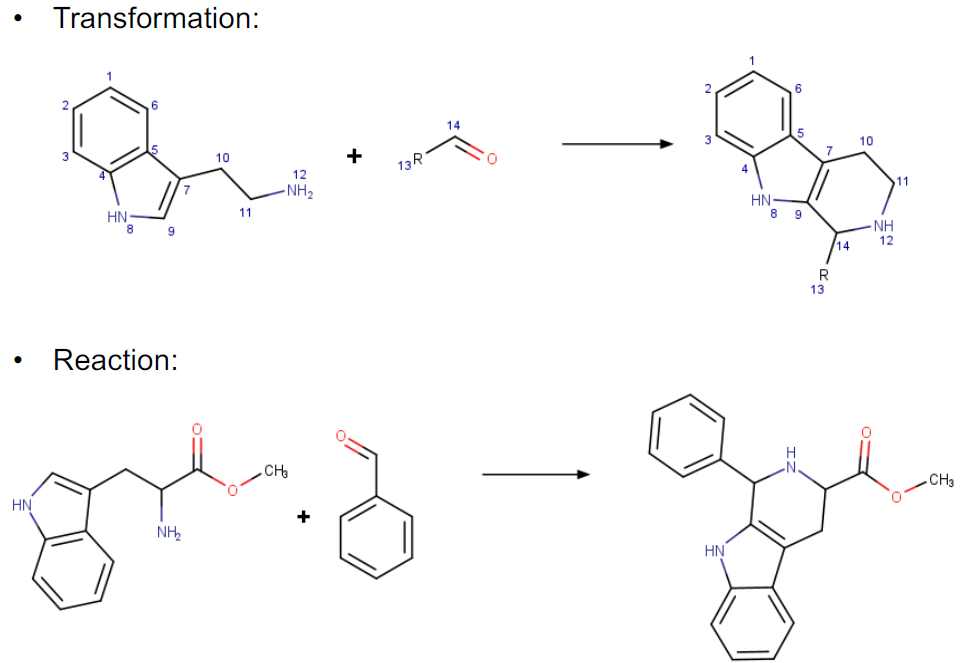
\includegraphics[width=0.75\textwidth]{img/cheminformatics/ChemicalReactionsTransformation.png}\end{center}

\paragraph{Reaction SMILES}
One way of representing reactions is Reaction SMILES, which extends SMILES to include various molecules separated by “.” and reaction direction by “$>>$”. Examples of nucleophilic substitution reactions can be seen below. 

\begin{itemize}
    \item C=CCBr.[Na]I$>>$C=CCI.[Na]Br
    \item C1CCCCC1Br.[Na]I$>>$C1CCCCC1I.[Na]Br
    \item C=CC(C)Br.[Na]I$>>$C=CC(C)I.[Na]Br
\end{itemize}

\paragraph{SMIRKS}
For database searches, generic reaction patterns must also be embedded, which can be done with SMIRKS, which is a combination of SMILES, SMARTS and atom mapping. However, the disadvantage of SMIRKS is that it can only be automated to a limited extent and is usually still created manually. The following rules apply:

\begin{itemize}
    \item Same number and type of mapped atoms on both sides
    \item Pairwise atom maps
    \item Non-mapped atoms may be deleted/created during reaction
    \item 1-1 stochiometry
    \item Explicit hydrogens must be mapped and appear on both sides
    \item Bond expressions must be valid SMILES
    \item Atom expressions either valid
\end{itemize}

\begin{center}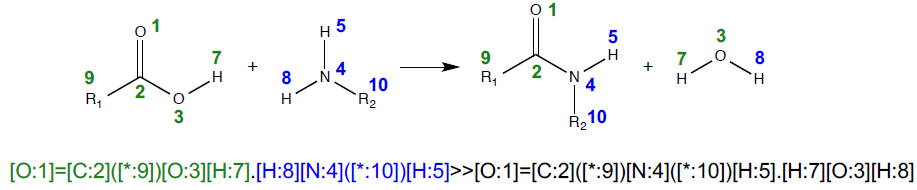
\includegraphics[width=0.75\textwidth]{img/cheminformatics/ChemicalReactionsSmirks.png}\end{center}

\paragraph{Atom Mapping}
The central concept in the digitization of reactions is atom mapping, because without atom mapping, incorrect results can be obtained. The problem, however, is that the mapping is only straightforward for simple and balanced reactions, but very few reactions are balanced. Since atom mapping is the most challenging task in this process, a tool that maps at least 85\% correctly is considered good.

\paragraph{Reaction Center}
Another approach is to focus only on the reaction center, i.e. those atoms and bonds that are directly involved in the bond formation or electron rearrangement. There are two main approaches for algorithms:

\begin{itemize}
    \item \emph{Based on common maximum substructure (MCS)}
    \begin{itemize}
        \item Find unchanged parts and derive reaction center (changed parts).
    \end{itemize}
    \item \emph{Optimizing the number of bonds broken and formed}
    \begin{itemize}
        \item Find reaction center (changed parts) and derive the unchanged parts.
    \end{itemize}
\end{itemize}

\subsection{Dimensionality reduction}

The problems we consider in chemistry and biology are usually high-dimensional, but not all dimensions are always needed for each solution. To solve the complexity of a problem in principle, it may therefore be useful to reduce the dimensionality of the problem. Dimensionality reduction can be very helpful when working with molecular fingerprints. This data transformation can be linear or non-linear, some methods being the following:

\begin{itemize}
    \item Principal component analysis (PCA)
    \item Factor analysis
    \item Multidimensional scaling (MDS)
    \item Isomap
    \item Local linear embedding
\end{itemize}

\subsubsection{Principal component analysis (PCA)}

PCA is a linear data transformation that maximizes the variance of the data in the lower-dimensional representation. This allows data sets of ratio-scaled variables to be simplified and visualized by approximating a large number of statistical variables by a smaller number of meaningful linear combinations (the principal components). In principle, PCA can be used for all dimensionalities, but in the following procedure we show PCA for two dimensions:

\begin{enumerate}
    \item For each dimension/variable, calculate the deviation from the mean.
    \begin{align}
        &x_i^\prime=x_i-\bar{x}&y_i^\prime=y_i-\bar{y}
    \end{align}
    \item Calculate the N-dimensional \emph{covariance matrix}.
    \begin{align}
        &C(x,y)=\begin{bmatrix}\mathrm{var}(x) & \mathrm{cov}(x,y)\\\mathrm{cov}(y,x) & \mathrm{var}(y)\end{bmatrix}&\begin{cases}
            \mathrm{var}(x)&\displaystyle=\frac{1}{N-1}\sum_{i=1}^{N}\left(x_i-\bar{x}\right)^2\\
            \mathrm{cov}(x,y)&\displaystyle=\frac{1}{N-1}\sum_{i=1}^{N}\left(x_i-\bar{x}\right)\left(y_i-\bar{y}\right)
        \end{cases}
    \end{align}
    \item Calculate the eigenvalues and (unit) eigenvectors of the covariance matrix.
    \begin{itemize}
        \item Eigenvalues are ordered by decreasing size.
        \item The larger the eigenvalue the more important is its corresponding eigenvector (= principal component).
    \end{itemize}
    \item Pick the $K$ largest eigenvalues to form the feature vector.
    \item Transform the data using the feature vector.
\end{enumerate}

\begin{center}
    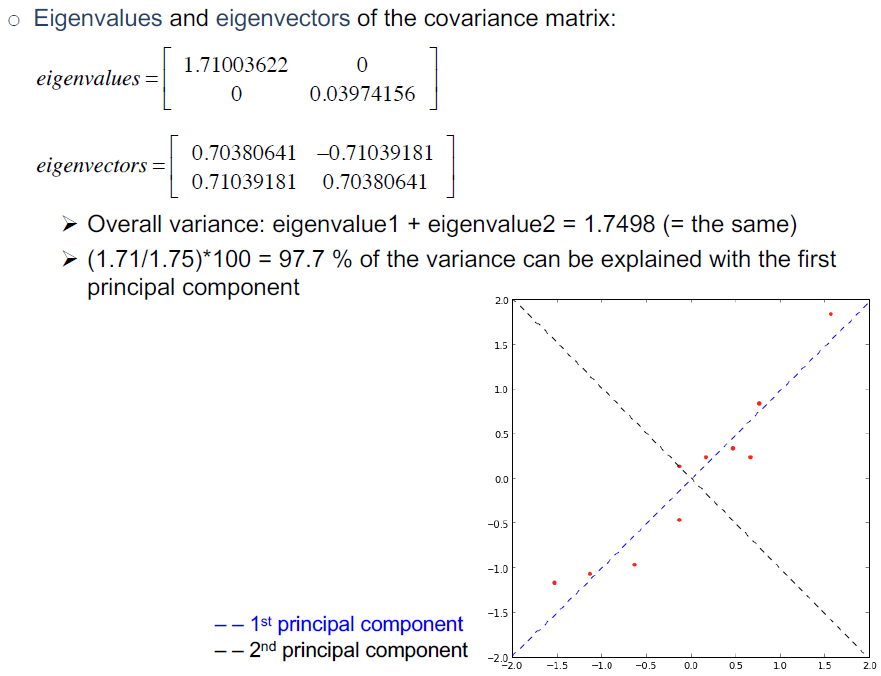
\includegraphics[width=0.45\textwidth]{img/cheminformatics/DimensionalityReduction1.png}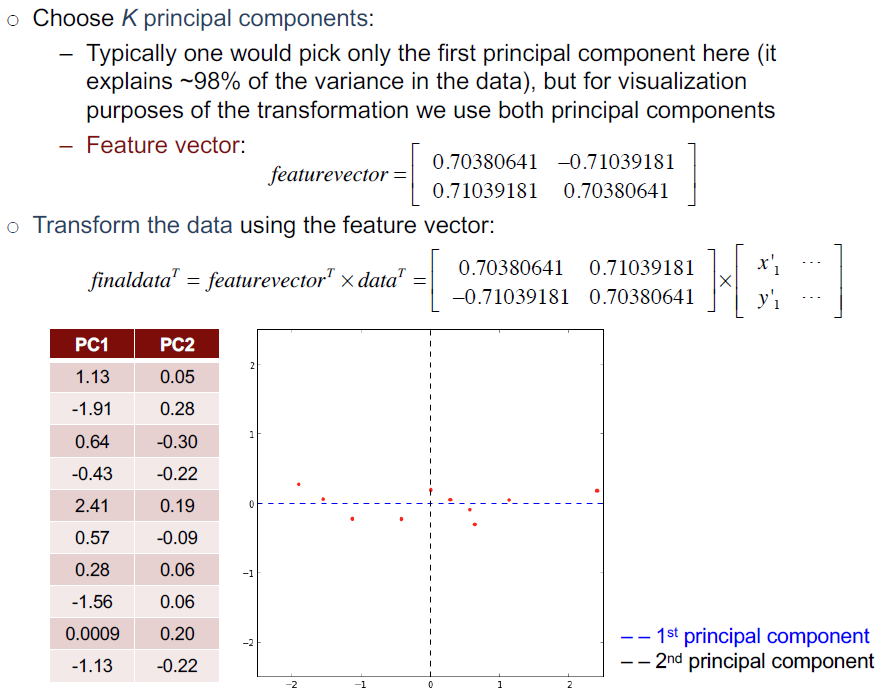
\includegraphics[width=0.45\textwidth]{img/cheminformatics/DimensionalityReduction2.png}
\end{center}

\subsection{Maximum Common Substructure (MCS)}

The problem of \emph{Maximum Common Substructure} (MCS) is to find the largest substructure from two or more structures. This can refer to a maximum number of atoms (MCIS: maximum common induced subgraph) or a maximum number of bonds (MCES: maximum common edge subgraph).

\begin{center}
    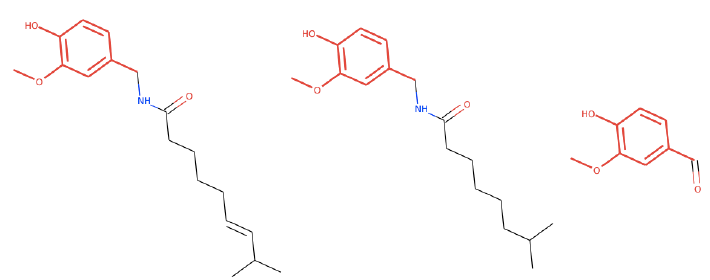
\includegraphics[width=0.85\textwidth]{img/cheminformatics/McsExample.png}
\end{center}

The MCS itself can also be approximate or exact and connected or not connected. However, MCS is an \emph{NP-complete} problem, which is why in the worst case the algorithms run exponentially. However, as is so often the case, molecular graphs allow for some heuristics that can significantly reduce the running times. Algorithmically, the problem can be solved exactly or approximately for connected MCS, as can be seen in the following list:

\begin{itemize}
    \item \emph{Exact algorithms}
    \begin{itemize}
        \item Maximum-clique based algorithms
        \item Backtracking
        \item Dynamic programming
    \end{itemize}
    \item \emph{Approximate algorithms}
    \begin{itemize}
        \item Genetic algorithms
        \item Combinatorial optimization
        \item Fragment storage
        \item Ad hoc procedures
    \end{itemize}
\end{itemize}

\subsubsection{Maximum Clique Problem}

The MCS problem can be reformulated as another classical NP-complete problem in graph theory, the \emph{Maximum Clique Problem}. For this purpose, the \emph{association graph} $G_\mathrm{A}$ is introduced from the two graphs $G_1$ and $G_2$, which makes an association vertex for each matching vertex pair of $G_1$ and $G_2$. The vertices in $G_\mathrm{A}$ are then connected if the adjacency of the corresponding vertex pairs are the same in $G_1$ and $G_2$. The \emph{clique} is now a complete subgraph of $G_\mathrm{A}$ (all nodes are connected to each other). This clique is then automatically the MCS of the two graphs $G_1$ and $G_2$.

\begin{center}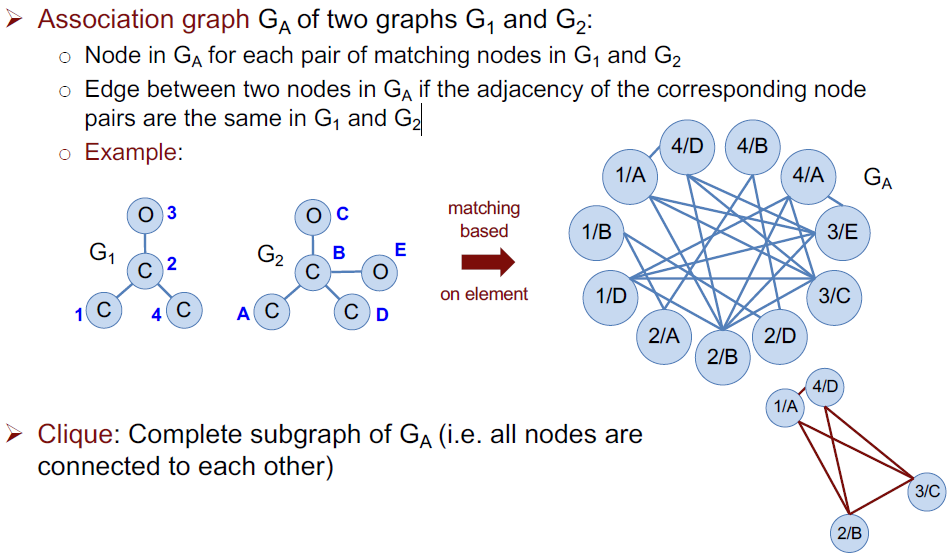
\includegraphics[width=0.85\textwidth]{img/cheminformatics/McsAssociationGraph.png}\end{center}

\paragraph{Bron-Kerbosch algorithm}

One algorithm for finding the maximum clique in such an associative graph is the \emph{Bron-Kerbosch} algorithm, which was presented in 1973 and is based on \emph{recursive backtracking}. For molecular graphs, heuristics can be used to reduce the size of the associative graph, for example by including element, hybridization and variant in the atom labels. These adaptations to the Bron-Kerbosch algorithm were presented in the \emph{SIMCOMP} algorithm in 2003. The edge weight of the associative graph can then be based on a full match with respect to atom labels or only a partial match. The search tree can also be processed using a greedy algorithm. The extension of the atom labels in the SIMCOMP algorithm introduced 68 atom types, which are shown below.

\begin{center}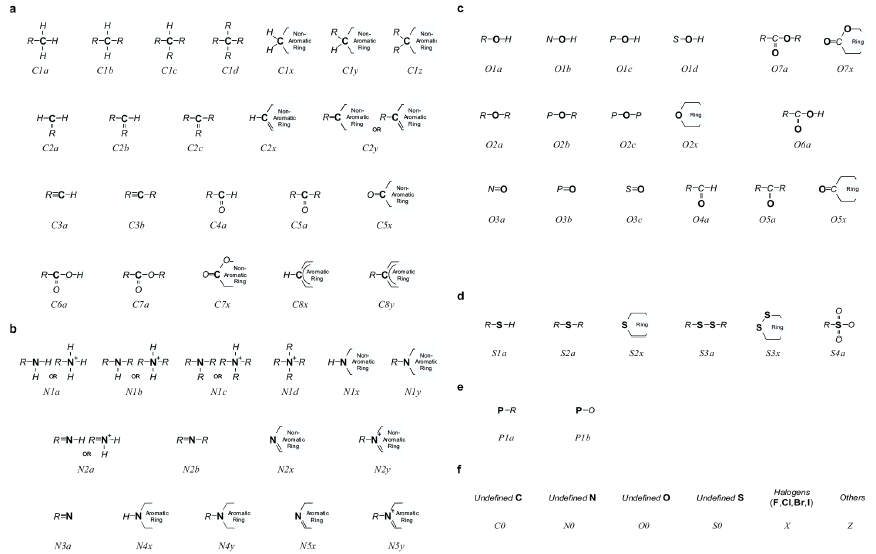
\includegraphics[width=0.85\textwidth]{img/cheminformatics/McsSimcompAtoms.png}\end{center}

\begin{enumerate}
    \item Calculate the association graph $AG$ of two initial graphs $G_1$ and $G_2$:
    \begin{itemize}
        \item Each vertex of AG corresponds to each atom-match of any possibilities with a proper weight (black: w = 1, grey: w = 0.5)
    \end{itemize}
    \begin{center}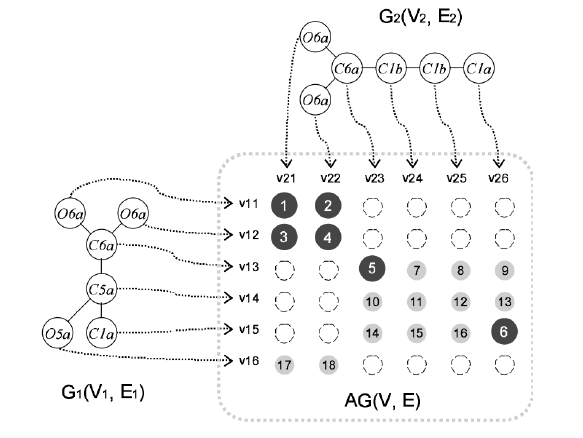
\includegraphics[width=0.85\textwidth]{img/cheminformatics/McsSimcompAlgorithm1.png}\end{center}
    \item Find maximum clique in AG:
    \begin{itemize}
        \item Maximize number of matched atoms
        \item Normalized score (Tanimoto coefficient):
        \begin{align}
            S_\mathrm{Tanimoto}=\frac{|MCS(G_1, G_2)|}{|G_1|+|G_2|-|MCS(G_1,G_2)|}
        \end{align}
    \end{itemize}
    \item With a maximum clique at hand, generate atom-matching list in original graphs (atom alignment):
    \begin{center}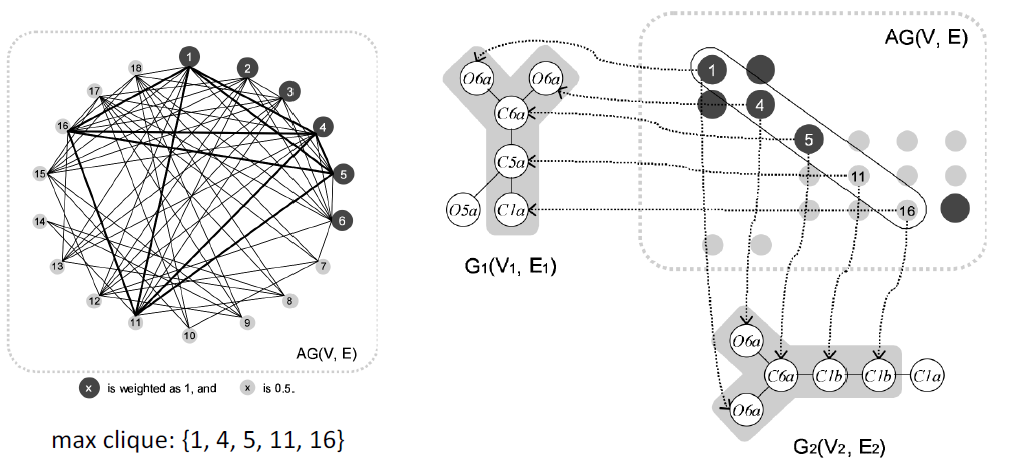
\includegraphics[width=0.85\textwidth]{img/cheminformatics/McsSimcompAlgorithm3.png}\end{center}
\end{enumerate}

% not finished code
%\lstinputlisting[language=C++]{src/cheminformatics/bronKerbosch.cpp}



\subsection{Scaffolds}

\subsection{Generation of 3D coordinates}

\subsubsection{Distance geometry}

\subsection{Clustering}

\subsubsection{Hierarchical}

\subsubsection{Application to chemical space}

\subsubsection{Non-hierarchical}

\subsubsection{Application to conformations}